\RequirePackage{xcolor}
\documentclass[journal,twoside,web]{ieeecolor}
\usepackage{jsen}
\usepackage{cite}
\usepackage{amsmath,amssymb,amsfonts}
%\usepackage{algorithmic}
\usepackage{graphicx}
\usepackage{textcomp}
\usepackage{wrapfig}
\usepackage{amssymb}
\usepackage{xcolor}
%\usepackage{cite}
%\usepackage[cmex10]{amsmath}
\usepackage{algorithmic}
\usepackage{array}
\usepackage{stfloats}
\usepackage{url}
%\usepackage{wrapfig}
%\usepackage{graphicx}
\usepackage{epstopdf}
\usepackage{subfigure}
\usepackage{epsfig}
\usepackage{tikz}
\usepackage{dcolumn}
\usepackage{bm}
\usepackage{color}
%\usepackage{amsmath}
\usepackage{accents}
\usepackage{braket}
\usepackage{mathtools}
\usepackage{tabularx}
\usepackage{nicefrac}
\usepackage{booktabs}
\usepackage{array}
\usepackage{multirow}
%\usepackage{xcolor}
\usepackage[geometry]{ifsym}
%\usepackage{textcomp}
%\usepackage{amsmath}
\usepackage[T1]{fontenc}
%\usepackage{tikz}
%Definition of donde se dejan las imagenes
\graphicspath{ {./images/} }
%Definition colour comments
\definecolor{javcolor}{rgb}{1.00, 0.0, 0.00}
\newcommand{\javnote}[1]{\textcolor{javcolor}{#1}}
%Definition colour
\definecolor{inicolor}{rgb}{0.0, 0.0, 1.00}
\newcommand{\ininote}[1]{\textcolor{inicolor}{#1}}
\definecolor{inacolor}{rgb}{0.0, 1.0, 1.00}
\newcommand{\inanote}[1]{\textcolor{inacolor}{#1}}
\newcommand*{\tikzbullet}[2]{%
  \setbox0=\hbox{\strut}%
  \begin{tikzpicture}
    \useasboundingbox (-.2em,0) rectangle (.2em,\ht0);
    \filldraw[draw=#1,fill=#2] (0,0.3\ht0) circle[radius=.2em];
  \end{tikzpicture}%
}
\newcolumntype{N}{>{\centering\arraybackslash}m{.5in}}
\newcolumntype{M}{>{\centering\arraybackslash}m{0.7in}}
\newcolumntype{G}{>{\centering\arraybackslash}m{2in}}
\newcommand{\markerone}{\raisebox{0.5pt}{\tikz{\node[draw,scale=0.4,circle,fill=black!20!blue](){};}}}
\newcommand{\markertwo}{\raisebox{0pt}{\tikz{\node[draw,scale=0.3,regular polygon, regular polygon sides=3,fill=black!45!green,rotate=180](){};}}}
\newcommand{\markerthree}{\raisebox{0.5pt}{\tikz{\node[draw,scale=0.3,regular polygon, regular polygon sides=3,fill=black!10!red,rotate=0](){};}}}
\newcommand{\markerfour}{\raisebox{0.5pt}{\tikz{\node[draw,scale=0.4,regular polygon, regular polygon sides=4,fill=none](){};}}}
\newcommand{\markerfive}{\raisebox{0pt}{\tikz{\node[draw,scale=0.4,diamond,fill=black!10!gray](){};}}}
\newcommand{\markersix}{\raisebox{0.6pt}{\tikz{\node[draw,scale=0.3,circle,fill=black!100!](){};}}}

\def\BibTeX{{\rm B\kern-.05em{\sc i\kern-.025em b}\kern-.08em
    T\kern-.1667em\lower.7ex\hbox{E}\kern-.125emX}}
\markboth{\journalname, VOL. XX, NO. XX, XXXX 2022}
{Author \MakeLowercase{\textit{et al.}}: Preparation of Papers for IEEE TRANSACTIONS and JOURNALS (February 2017)}
\definecolor{abstractbg}{rgb}{0.89804,0.94510,0.83137}
\setlength{\fboxrule}{0pt}
\setlength{\fboxsep}{0pt}
\begin{document}
\title{Highly sensitive undersea corrosion monitoring system}
\author{Javier Alonso-Valdesueiro, \IEEEmembership{Member, IEEE}, I\~naki Madinabeitia, I\~nigo Santos-Pereda, Jean-Baptiste Jorcin, and Esther Acha-Pe\~na
\thanks{This project  has  been funded by the Government of the Basque Country through the HAZITEK project ref. ZE-2019/00028 of Department of Economic Development and Infrastructure.}
\thanks{J. Alonso-Valdesueiro is with TECNALIA, Basque Research and Technology Alliance (BRTA),Mikeletegi Pasealekua 2, 20009, Donostia-San Sebastián, Spain (e-mail: javier.alonso@tecnalia.com). }
\thanks{I. Madinabeitia, is with TECNALIA, Basque Research and Technology Alliance (BRTA),Mikeletegi Pasealekua 2, 20009, Donostia-San Sebastián, Spain (e-mail: inaki.madinabeitia@tecnalia.com).}
\thanks{I. Santos, was with TECNALIA, Basque Research and Technology Alliance (BRTA),Mikeletegi Pasealekua 2, 20009, Donostia-San Sebastián, Spain (e-mail: inigo.santos@outlook.es).}
\thanks{J.B. Jorcin is with TECNALIA, Basque Research and Technology Alliance (BRTA),Mikeletegi Pasealekua 2, 20009, Donostia-San Sebastián, Spain (e-mail: jbaptiste.jorcin@tecnalia.com).}
\thanks{E. Acha-Pe\~na University of the Basque Country (UPV/EHU), Ingeniero Torres Quevedo Plaza, 1, 48013 Bilbao, Biscay, Spain (e-mail: esther.acha@ehu.eus).}}

\IEEEtitleabstractindextext{%
\fcolorbox{abstractbg}{abstractbg}{%
\begin{minipage}{\textwidth}%
\begin{wrapfigure}[15]{r}{3in}%
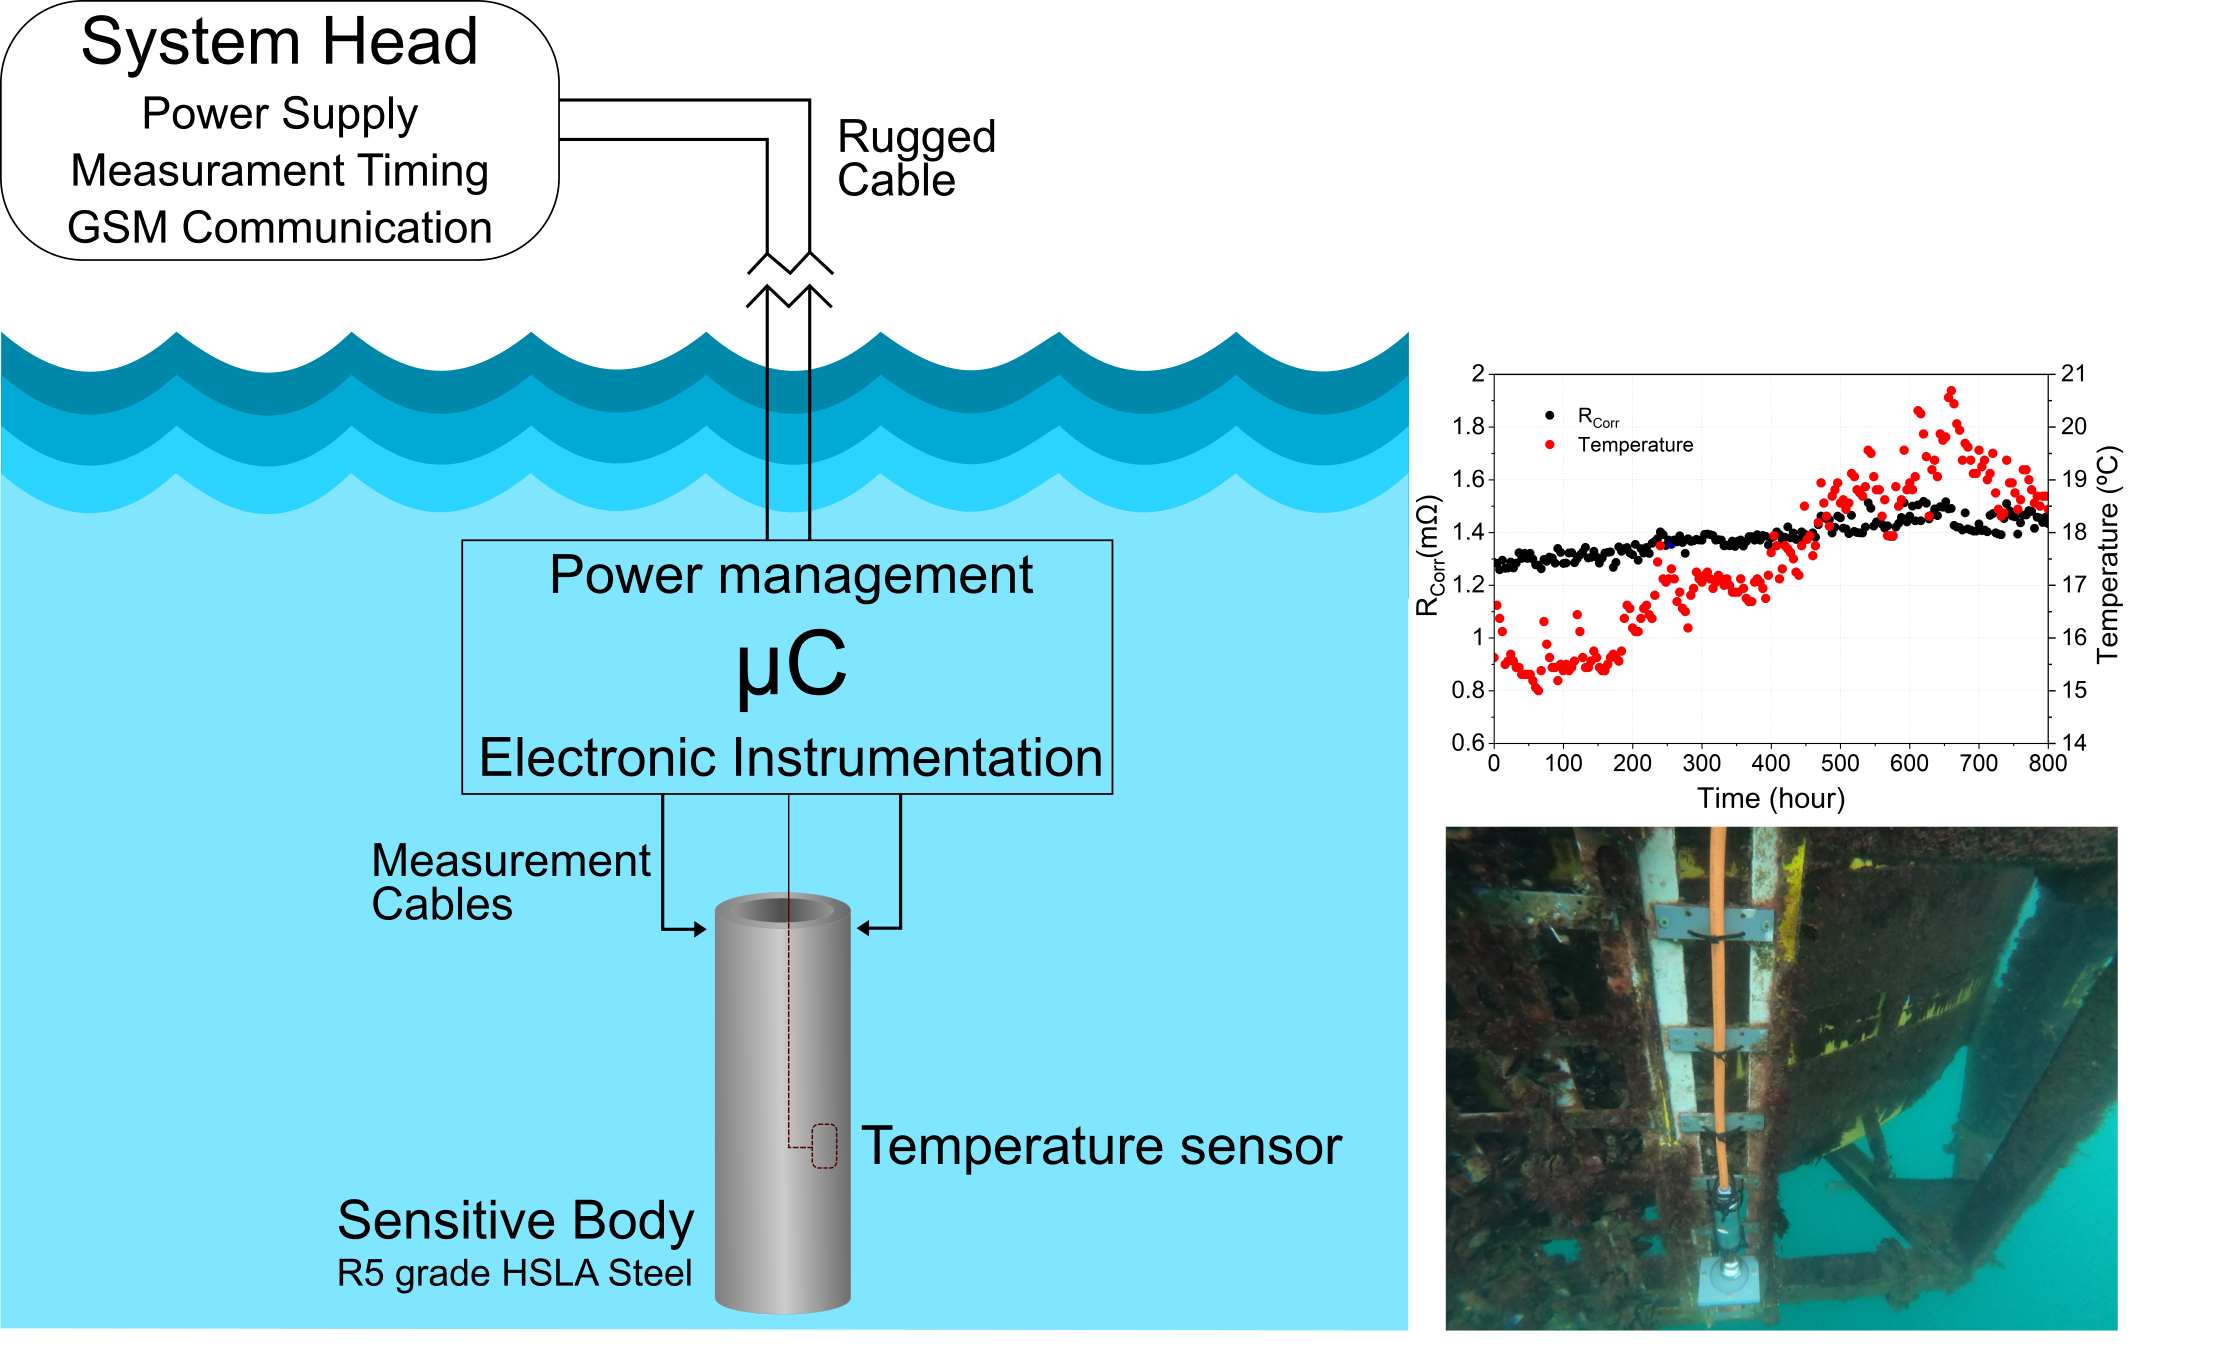
\includegraphics[width=3in]{images/TOC_v1.png}%
\end{wrapfigure}%
\begin{abstract}
Corrosion monitoring of undersea metallic structures has become one of the major challenges for the energy industry in the last two decades. Reliability, autonomy and high grade of accuracy is expected from a network of sensors distributed along subsea distribution grids and maintenance equipment. Despite the many techniques proposed by the scientific literature, the most extended techniques rely on the corrosion of low and ultra-low resistive elements with degradation rates similar to the metallic structures under monitoring, more commonly known as corrosion probes. However, the sensitivity of resistive sensors is limited to $25\,\nicefrac{\mu m}{yr}$ in a time frame of $10$ days which reduces the time response of the sensor to fast corrosion process. The most extended solution is to decrease the thickness of the resistive element. This solution increases the resolution by increasing the resistance of the resistive element and the influence of any material reduction due to corrosion. However, a decrease in thickness leads to shorter lifetimes and a higher influence of thermal variations. In this work, a highly sensitive resistive corrosion sensor and its performance are presented. The functionality of a highly sensitive $\mu$Ohm-meter as a corrosion sensor and its uncertainty in corrosion rate are analyzed. Different sensor prototypes for laboratory and field deployment are described thoroughly and tested for calibration purposes in corrosive environments. The final prototype is connected to an autonomous platform and deployed in an offshore platform located at the Cantabrian Sea resulting in a corrosion rate sensitivity of $\sim$\,$1.1\,\nicefrac{\mu m}{yr}$ in $4$\,hours time frame.
\end{abstract}

\begin{IEEEkeywords}
Low Resistance Measurements, Corrosion monitoring, undersea facilities, internet of things.
\end{IEEEkeywords}
\end{minipage}}}

\maketitle

\section{Introduction}
\label{sec:intro}
\IEEEPARstart{M}{onitoring} the integrity of undersea parts and devices has become one of the most important issues in offshore facilities during the last decade~\cite{yang2018, coelho2017, islam2015, singh2014, yasri2014, diler2014, yu2010}. Particularly,  seawater corrosion monitoring has recently turned into one of the trending topics in the energy sector~\cite{zakowski2014, alcantara2017} due to recent environmental catastrophes and failures. Therefore, energy companies have focused their attention on stand-alone sensor networks working in undersea environments devoted to corrosion monitoring~\cite{martinez2016, johny2016, beganovic2015, agarwal2014,xu2014}.


Scientific literature shows an increasing effort on developing feasible corrosion sensors by applying different techniques~\cite{wright2019}. However, despite the variety of these techniques (covering from optical devices~\cite{coelho2017,islam2015} to biologic structures~\cite{diler2014}),
commercial sensors are mostly based on monitoring the small resistance of a piece of metal (the body) immerse in a corrosive environment such as saltwater~\cite{prosek2014}. They are typically called Electrical Resistance (ER) sensors~\cite{mcKenzie1985} and they are widespread because of the information they provide about mass loss due to corrosion. This body mass loss vs time provides information of the corrosion rate for a specific material and corrosive environment.

However, despite their advantages, ER sensors present two main problems to overcome. First, high sensitivity in ER sensors is commonly achieved by a small thickness of the body (either the wall of a tube or the thickness of a filament). At the same time, a long service time is achieved by increasing the thickness of the body. As the sensitivity of the sensor is limited by the smallest resistance the electronics are able to measure, the thickness of the body is, therefore, limited by this measurement constraint and so it is the service time.

Second, a thermal gradient on the body of the ER sensor results in major deviations in accuracy and repeatability~\cite{reilly2018, corres2014, cross2011}.
Accordingly, commercial sensors include a reference body, placed out of the corrosive environment, which facilitates the deconvolution of the corrosion rate information from thermo-electric perturbations. However, literature reported that differences of $0.25^{\circ}$\,C between reference and sensitive bodies can lead to $1000$\,ppm deviations in resistance measurements~\cite{rhoades1986,p_rhoades1980,hilbert2006} which can be an unacceptable loss of accuracy in critical undersea facilities.

In this contribution, a highly sensitive ER sensor and its deployment in an offshore platform is presented. The ER sensor is built around $\mu$Ohm-meter based on the lock-in amplifier presented in~\cite{bengtsson2012} and the switching DC resistance measurement~\cite{schweiger2010}. The sensor also includes temperature sensors placed on the sensitive body in order to fine-tune the resistance measurement. This topology faces the two problems of ER sensors presented above. First, the developed $\mu$Ohm-meter provides higher resolution than the available commercial sensors, allowing thicker sensitive bodies and enlarging the service time. The lock-in amplifier technique implemented with a 16-bits ADC provides higher resolution in the resistance measurement and better reliability than 4-wire direct DC resistance measurement. Second, while the switching DC resistance is able to minimize the influence of the constant thermal-effects (Seebeck effect), the two temperature sensors provides enough information to correct the resistance measurement off-line and minimize the influence of a temperature gradient in the sensitive body. Finally, the necessary platforms for laboratory and field deployment are also presented in order to finally immerse the sensor autonomously in the Cantabrian Sea. 

The sensitive body placed in the sensor is a $1$\,mm thick HSLA steel tube, similar to the T40 probe form EuropCor, CT50 from MetalSamples and T50 from COSACO.  These cylindrical probes with the associated electronics ensure measurements of corrosion rates that ranges from $885$\,$\mu$m (T50) to $\sim90$\,$\mu$m (T40) when $4$ hours response time is consider. The sensitivity of the presented sensor ranges form $\sim0.5$\,$\mu$m to $\sim1.1$\,$\mu$m which are $\sim$\,$70$ times better than the presented commercial equipment. This result allows to the sensor network deployers span the service time without loosing response time and sensitivity. 


Accordingly, the paper is organised as follows: First, in section~\ref{sec:corrsens}, a general description of the sensor is provided. The block diagram of the device and the electronics in charge of the resistance measurements is depicted along with a description of the different subsystems. In section~\ref{sec:protytpes}, different versions of the block diagram mentioned above are presented and briefly discussed. The final system is described for both laboratory and \textit{in-field} operations. After that, in section~\ref{sec:resMeasCorrEnv} measurements of different corrosion rates are presented for different corrosive environments, including different solutions of \textit{Aqua Regia} (HNO$_{3}+3$HCl) and salt water, and compared with the theoretical performance of the sensor. Finally, in
section~\ref{sec:conclusions} Measurements in a real offshore platform are presented and discussed in comparison with laboratory results.

\section{High Sensitivity $\mu\Omega$-meter}
\label{sec:corrsens}
\subsection{System Block Diagram}
\label{ssec:sysBlockD}
Figure\,\ref{fig:senBlockD} shows the block diagram of the sensor when it is placed in seawater. The system includes a head (based on the Raspberry Pi platform) providing enough power to the system, communicating with the sensor electronics downstream by an RS485 bus and communicating data from the sensor electronics to an onshore facility via Global System for Mobile communications (GSM).

\begin{figure}[!t]
\centering
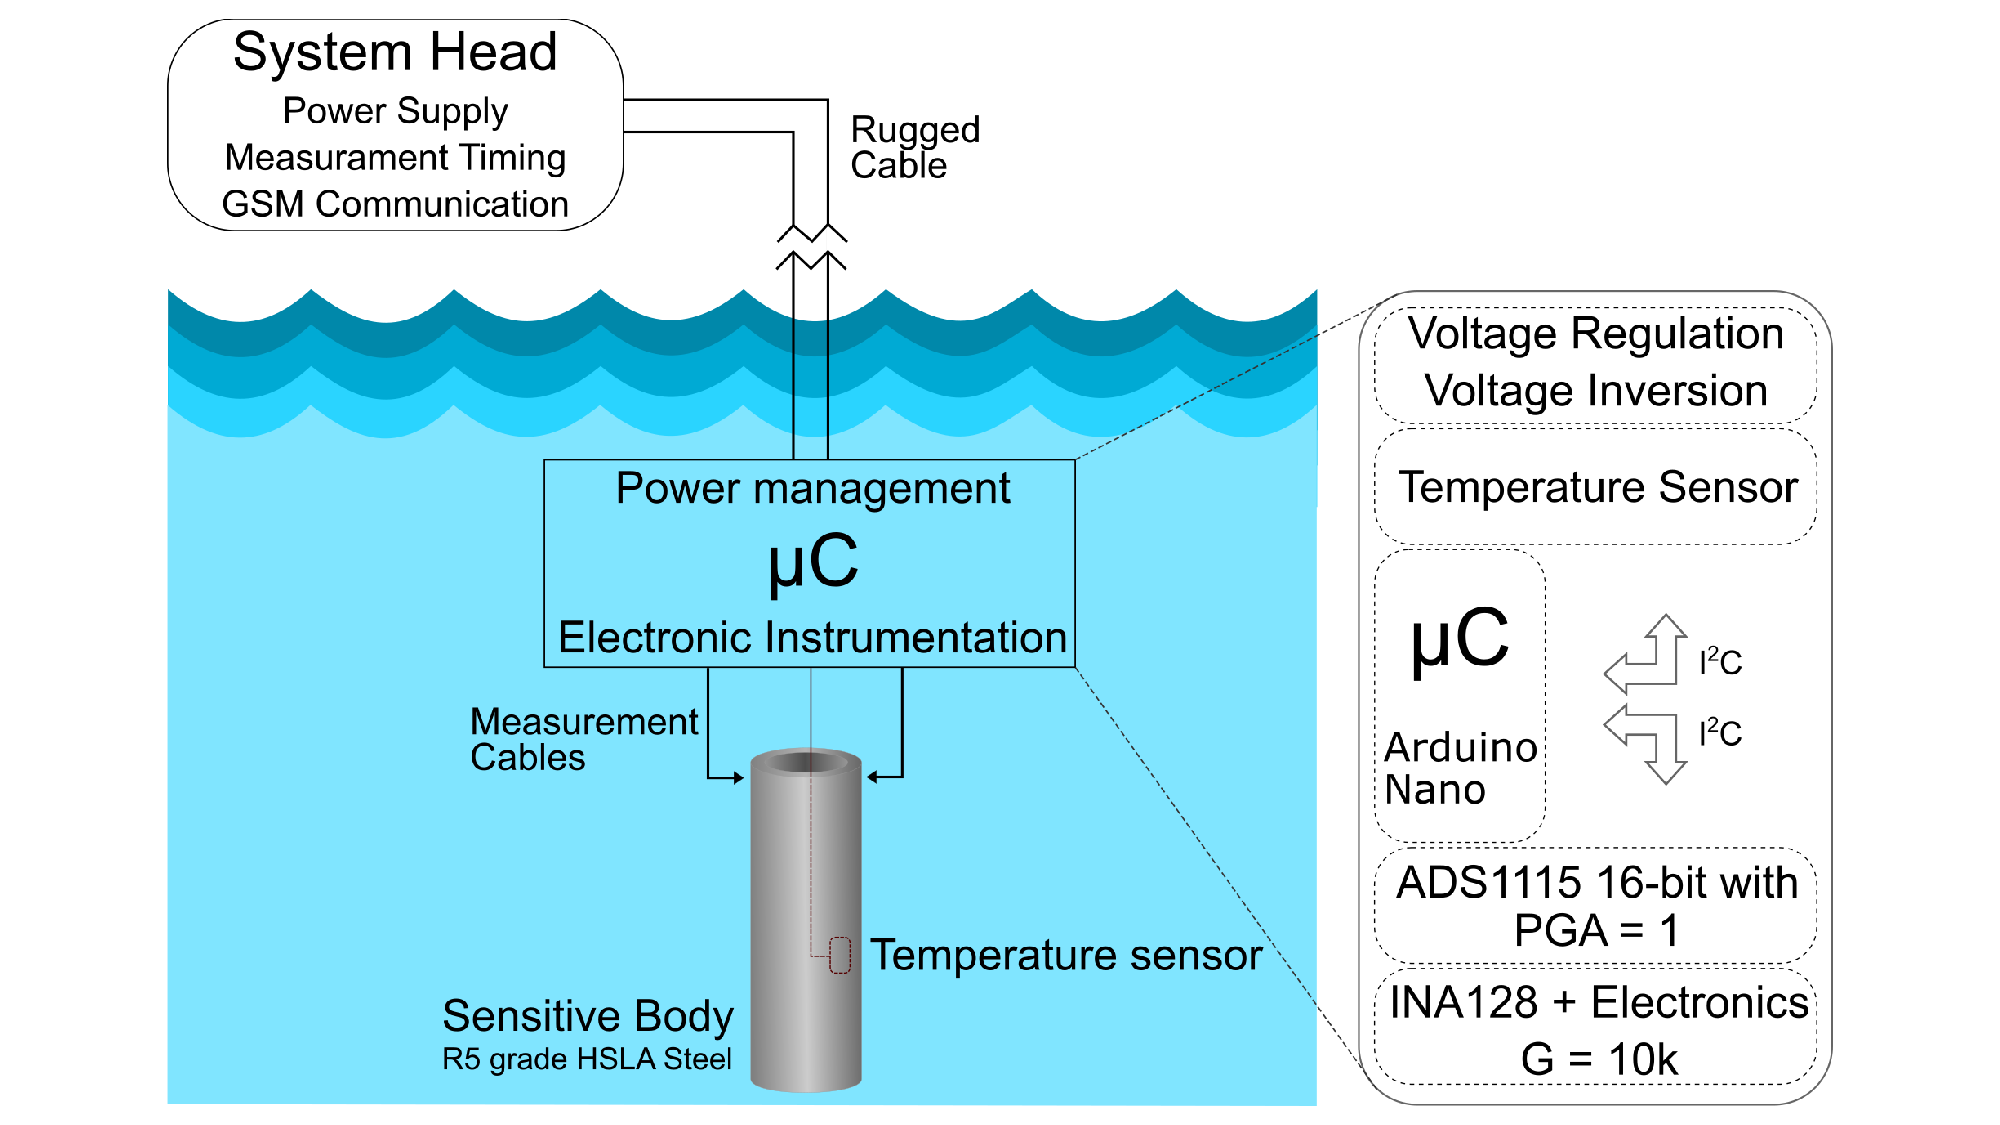
\includegraphics [trim = 25mm 0mm 25mm 0mm, clip, width=1\columnwidth]{images/fig1_v2.pdf}
\caption{Block diagram of the sensor developed for corrosion monitoring in seawater. The sensitive body is a R5 grade HSLA steel tube $150$\,mm long with $13$\,mm outer diameter and $12$\,mm inner diameter. A sensor is placed inside the body in order to control the temperature during measurements. The body is attached to the electronics described on the right side. The electronics include voltage regulation, temperature measurement of the electronics, and extra ADC ADS1115 and an INA128 amplifier responsible of resistance measurement. Communications and power are provided to electronics by a rugged cable connected to the head. This head is in charge of providing power to the system, managing the measurements with the ARDUINO ($\mu$C) and communicate with an onshore facility.}
\label{fig:senBlockD}
\vspace{-0.3cm}
\end{figure}

The power line and the RS485 bus are guided downstream by a rugged cable connecting with the sensor front-end. This front-end includes a voltage regulation to $10$\,V, a voltage inverter using a DC-pump ICL7660 and an RS485 transceiver SP3485 configured in half-duplex mode. Everything is attached to the ARDUINO Nano which obtains the temperature readings of the electronics by two DS18B20 sensors (one placed on the sensitive body and the other nearby the electronics) connected via $1$-\textit{Wire} protocol. Finally,  the ARDUINO Nano gets the resistance measurement from an ADC ADS1115 connected via I$^{2}$C bus. This measurement consists of a voltage amplified by an INA128 instrumentation amplifier whose gain is set to $10^{3}$. The ARDUINO transforms the voltage into resistance by a simple calculation. 

The body consists of a R5 grade HSLA steel tube $150$\,mm long with $13$\,mm and $12$\,mm outer and inner diameter respectively. The corrosion rate of this type of steel varies with the immersion time from $0.16$\,mmpy to $0.035$\,mmpy depending on the fouling load~\cite{palanichamy2014,blekkenhorst1986}. Therefore, $1$\,mm thickness of the tube wall should be enough to observe changes in the resistance during $1.5$ years or more with a $50\%$ safety margin.

\begin{figure}[!t]
\centering
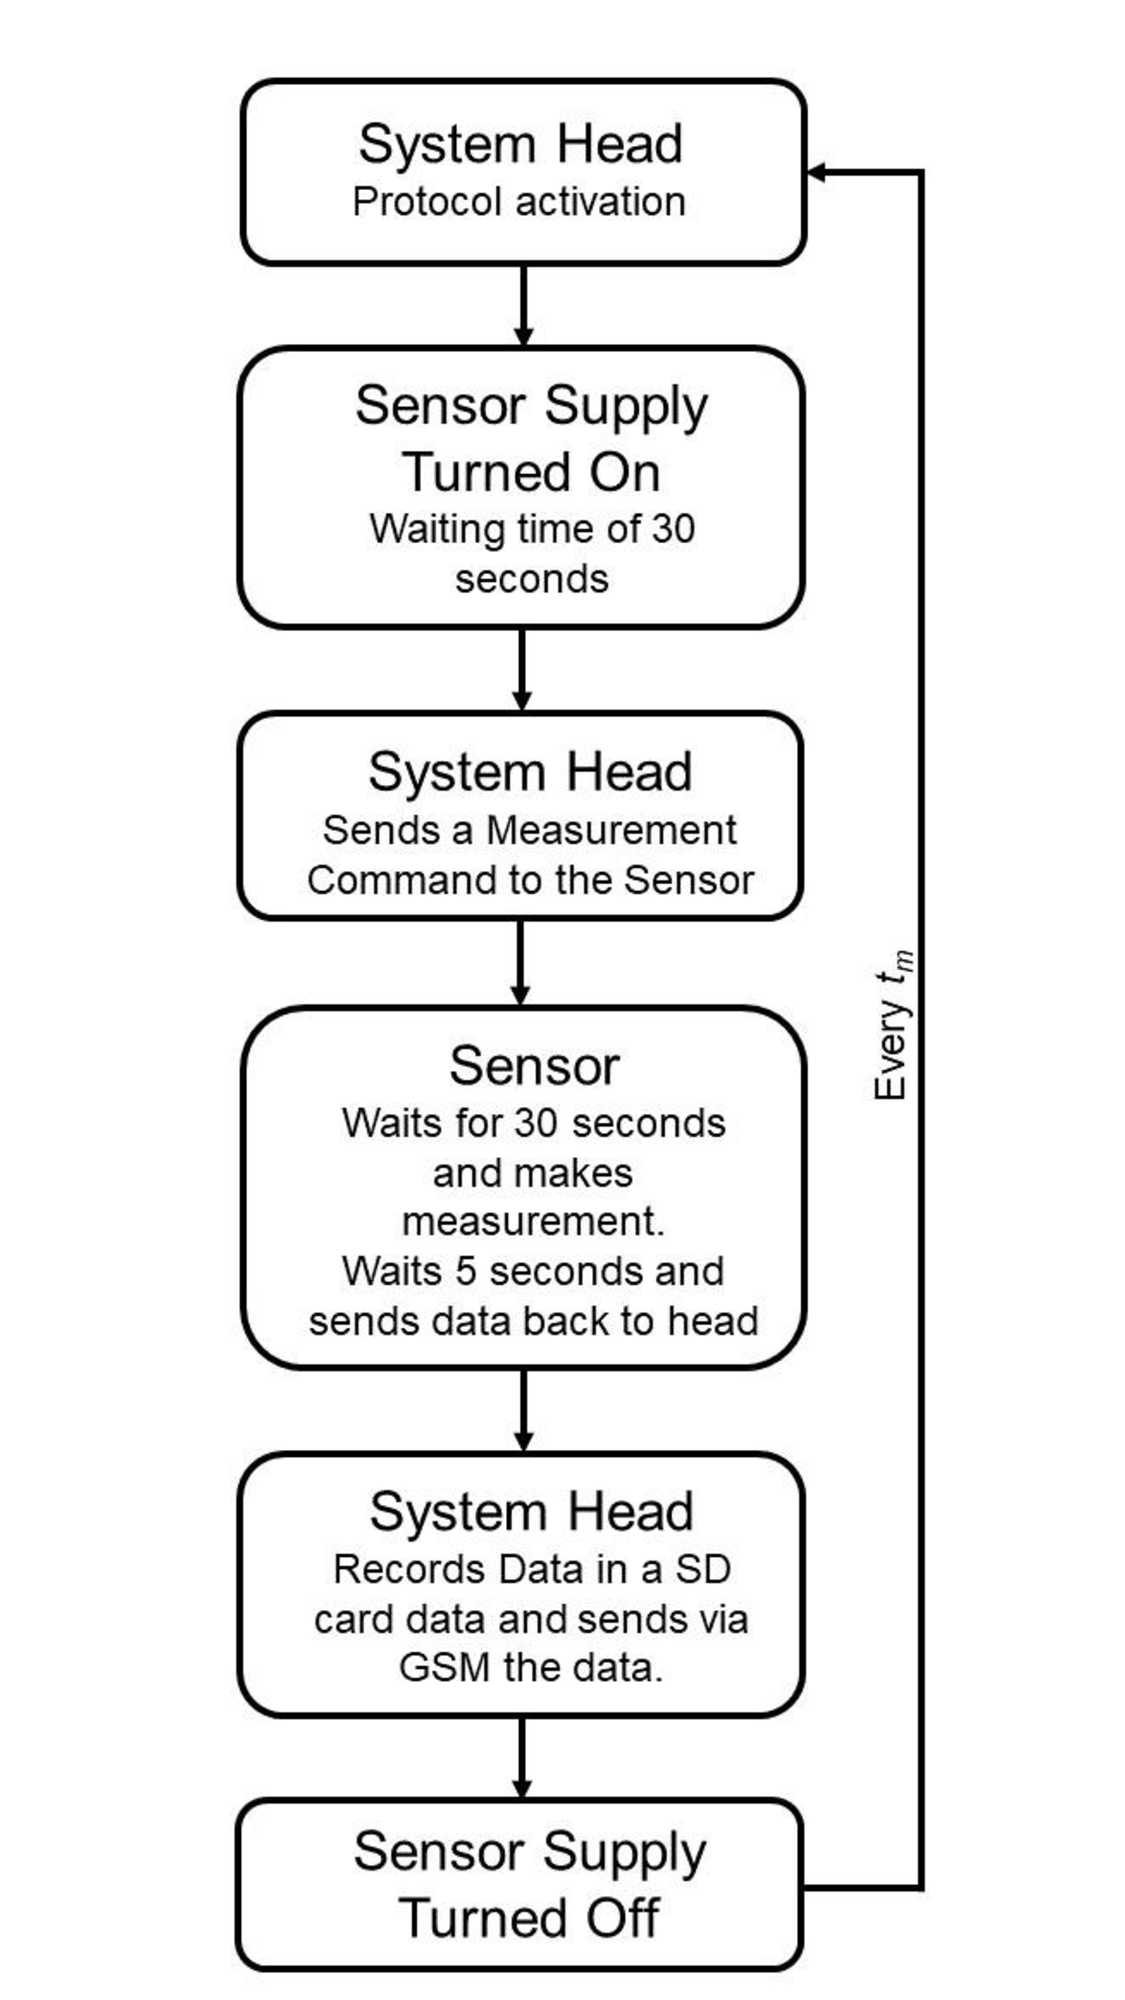
\includegraphics [trim = 35mm 0mm 20mm 10mm, clip, width=0.7\columnwidth]{images/fig2_2.pdf}
%\hfill
\caption{Flow diagram of the measurement protocol. Every \textit{t$_{m}$} the system head turns on the power supply of the sensor electronics by simply switching a relay connected to the $12$\,V battery. After $30$\,s the system head sends and ASCII character via RS485, starting the measurement algorithm in the Sensor $\mu$C. Whenever the $\mu$C finishes the measurement (typically a minute), it sends the data back to the system head. The system head checks for errors and records in an SD card added to the head. Finally it sends the data via GSM to a prefixed phone number. The system head powers off the sensor, ending the measurement cycle.}
\label{fig:typCorrSensor}
\vspace{-0.5cm}
\end{figure}
Figure\,\ref{fig:typCorrSensor} shows the measurement protocol activated by the head every \textit{t$_{m}$} which is programmable. The system head starts the protocol by powering up the sensor. The head switches a relay that connects the battery to the sensor via the rugged cable. The voltage from the battery is regulated to $12$\,V and boosted to $17$\,V by a DC booster. The peak current of the sensor during measurement is $\sim$\,$100$\,mA. After $30$\,s, the system head sends an ASCII character which indicates to the $\mu$C inside the sensor to start the measurement and waits for reply. If no reply comes back in $2$ minutes the system head sends a new ASCII character. If, after three attempts there is no response a failure mark is recorded in an SD card and sent via GSM to the onshore facility.

In the case of normal operation of the sensor, its $\mu$C waits for $30$\,s all the electronics to be stabilized and, afterwards, collects the resistance measurement and both temperatures (electronics and body). It packs the data and sends them back to the head via RS485. The process of measurement and communication takes about a minute to be completed. Once it is finished, the $\mu$C stands by for a new ASCII character from the head.

The system head receives the data and records it in the SD card. It checks the availability of the GSM connection with a prefixed phone number onshore and, if there is connection, sends the data to the base. After that, it switches off the power relay and waits for \textit{t$_{m}$} for a new measurement protocol to start.
\vspace{0.5cm}
\subsection{Measurement of the Body Resistance}
\label{ssec:resMeasProt}

\begin{figure}[!t]
\centering
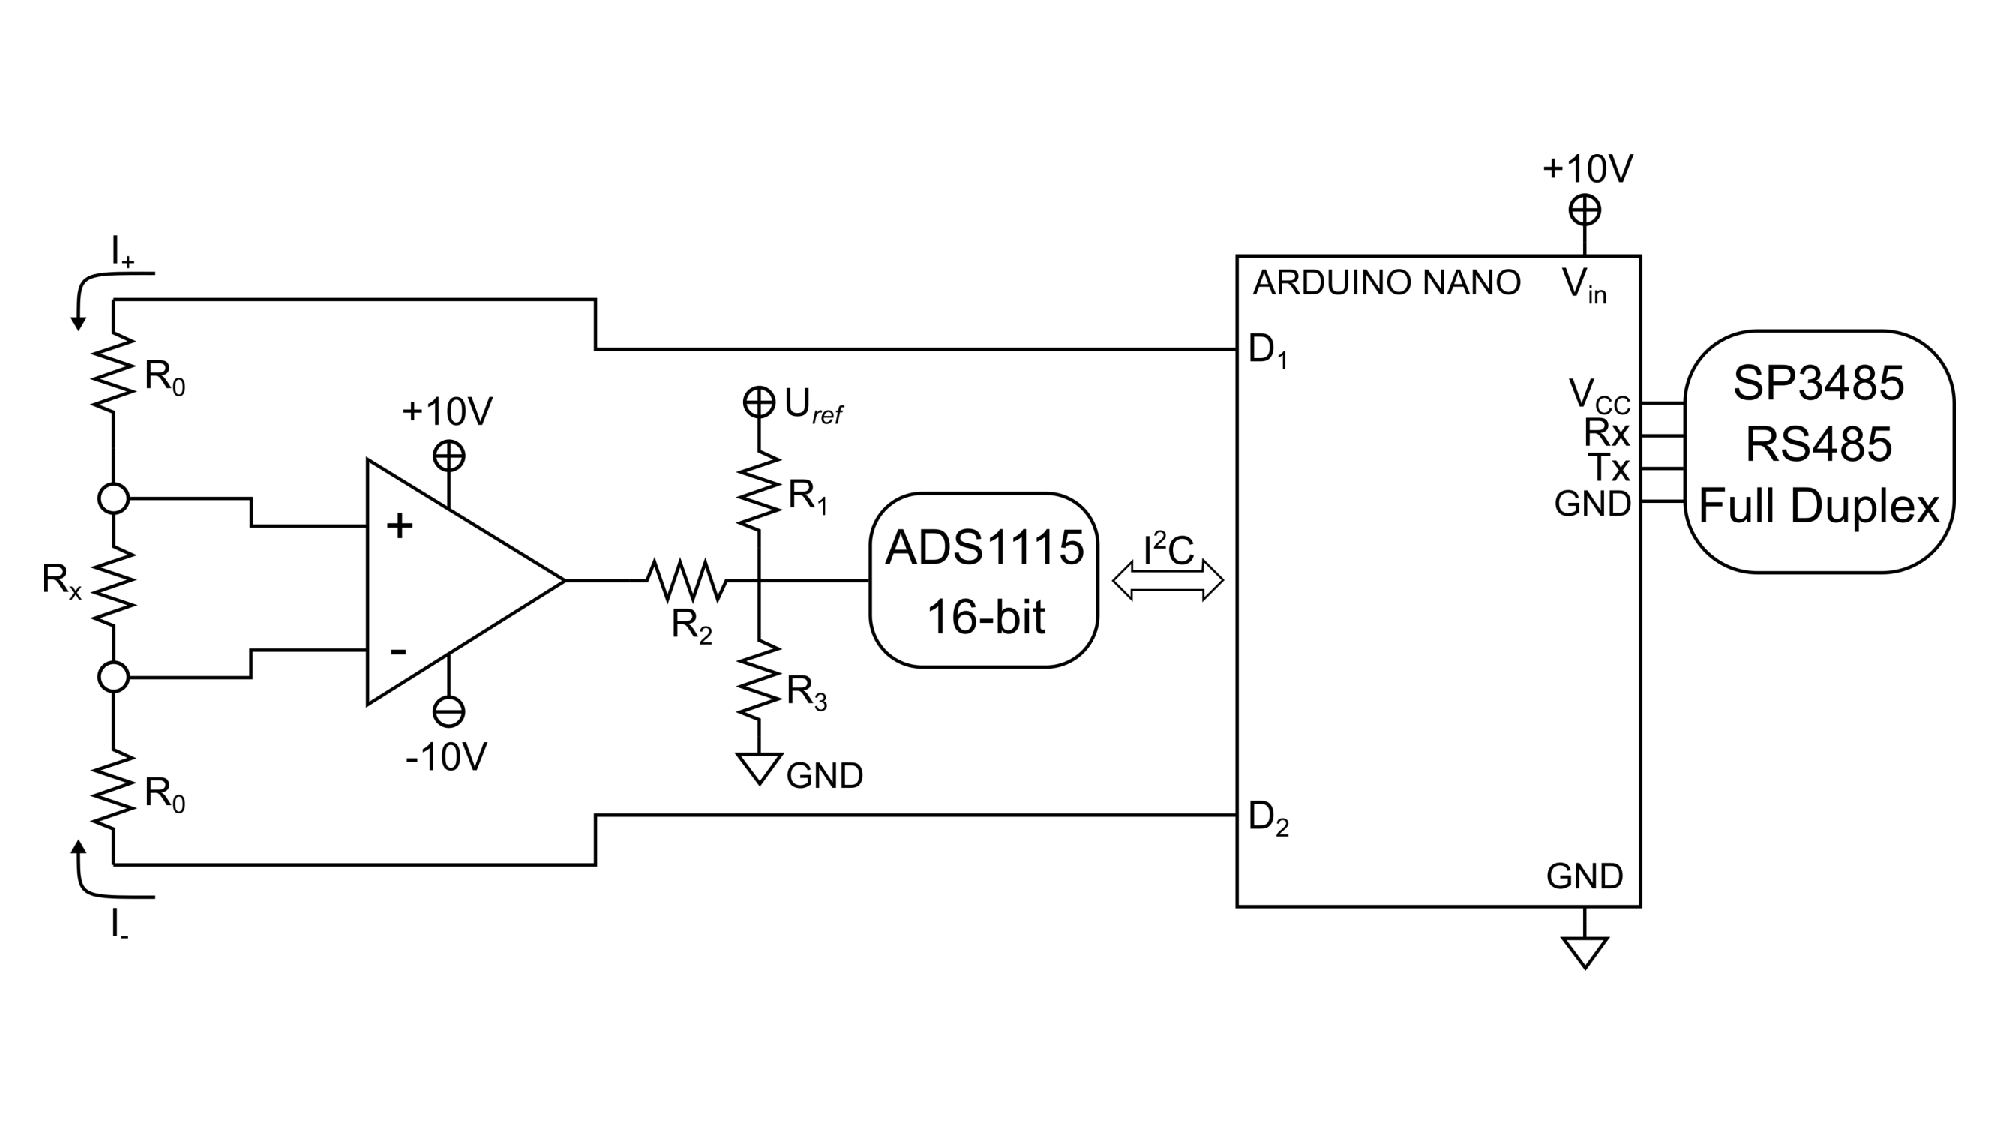
\includegraphics[trim = 0mm 0mm 0mm 0mm, clip, width=1\columnwidth]{images/fig3_V2.pdf}
\caption{Design of the electronics developed for the corrosion sensor. The design differs from the prototype presented in~\cite{bengtsson2012} in the presence of an ADC ADS1115 which increase the number of bits of the ADC to 16-bit and, therefore, increasing the resolution of the system by a factor of $64$. The plot also shows how the electronics are connected with the outside world via RS485 by connecting the SP3485 half Duplex IC with the ARDUINO Nano.}
\label{fig:resMeasProt}
\vspace{-0.3cm}
\end{figure}

Figure~\ref{fig:resMeasProt} shows the configuration of the instrumentation electronics devoted to measuring the resistance of the sensitive body.

Following the design presented in~\cite{bengtsson2012}, the sensitive body (R$_{x}$) is connected through 4 steel rods of $1.5$\,mm diameter welded to it. The resistance of the two rods connected to the current paths is added to R$_{0}$, which in this case is $150$\,$\Omega$ each. The resistance added to R$_{0}$ by the connection to the sensitive body (some AWG12 wire and the rods) is $\sim$\,$1.3$\,m$\Omega$. The other two rods are connected to the instrumentation amplifier in the same manner than the current paths.

Once the measurement starts, the ARDUINO Nano sets the digital output, D$_{1}$, to HIGH and the digital output D$_{2}$ to LOW. This produces a current I$_{+}=14$\,mA through the total resistance $2R_{0}+R_{x}$, where R$_{x}$ is the resistance of the body. The $\mu$C records the value provided by the ADC ADS1115 via I$^{2}$C after the INA128 stabilises its output. The gain of the INA is set to its maximum A$_{0}$ and the voltage coming into the ADC is pulled up by a resistor divider connected to the supply in order to place the voltage into the dynamic range of the ADS1115 ($0\rightarrow5$\,V). After that, the $\mu$C inverts the polarity of the digital outputs producing a current I$_{-}=-14$\,mA through the resistances and read from the ADC in the same manner than with I$_{+}=-14$\,mA.

The values provided by the ADC, s$_{+}$ and s$_{-}$, are substracted. The whole process is repeated N times and the final value, \textit{s}, is averaged in order to reduce the noise. note that all s$_{+}$, s$_{-}$ and \textit{s} are integer numbers from $0$ to $2^{n}$ where n is the number of bits of the ADC ($15$ in the case of the ADS1115). As s is the result of DC switched measurement of the resistance of the body, all relevant thermo-electric effects (mainly the Seebeck effect) are removed from the measurement. 

The resolution of the presented method is governed by the following equation:
\begin{equation}
\label{eq:resRx}
\Delta R_{x} = \frac{\left( R_{OH}+2R_{0}+R_{OL}\right)\times U_{ref}}{k\times\left( V_{OH}-V_{OL}\right)\times \left(A^{+}_{0}+A^{-}_{0}\right)}\times\frac{1}{2^{n}}
\end{equation}
where R$_{OH, OL}$ are the internal resistances of the ARDUINO Nano digital outputs when they are in HIGH and LOW states respectively (they were measured to be R$_{OH}+$R$_{OL}=57.143$\,$\Omega$), U$_{ref}$ is the maximum voltage at the entrance of the ADC which is fixed to $4.967$\,V, k is the coefficient dividing the voltage coming out from the INA128 coming from the combination of R$_{1, 2, 3}$ ($0.2534$ in this case), V$_{OH, OL}$ are the high and low voltages in the digital output of the $\mu$C ($4.923$\,V and $2.679$\,mV respectively) and A$^{+,-}_{0}$ are the positive and negative maximum gains of the INA128 (considered A$^{+,-}_{0}=10029$).

With the values specified above, the expected resolution of the Ohm-meter developed for the corrosion sensor is $\Delta$R$_{x}=1.08$\,$\nicefrac{\mu\Omega}{\hat{s}}$, where $\hat{s}$ is the integer number returned from the ADC to the ARDUINO. Therefore, the resistance measured by the design is given by the following equation:

\begin{equation}
\label{eq:totalRx}
R_{x} = 1.08 \times s \left[\mu\Omega\right]
\end{equation}

Equation~\ref{eq:totalRx} shows the effect of placing an ADC with 16-bit resolution. The resolution increases $\sim$\,$64$ times when the 16-bits are considered. Theoretically, this resolution potentially leads to monitoring corrosion rates of $\sim$\,$180$\,$\nicefrac{nm}{yr}$ when a resistivity of $450$\,$\mu\Omega\cdot$mm is considered for HSLA steels.

\subsection{Error in the Resistance Measurement}
\label{ssec:errorRmeas}

The theory of error analysis states that the uncertainty of a multivariable function is calculated as follows:
\begin{equation}
\label{eq:errorGen}
u_{f}^{2}=\sum_{j}\left(c_{j}x_{j}\right)^{2} 
\end{equation}
where \textit{u$_{f}$} is the uncertainty of the multivariable function \textit{f}, \textit{x$_{j}$} is the uncertainty of the \textit{j$_{th}$} variable of the function \textit{f} and \textit{c$_{j}$} is given by the partial derivative of \textit{f} with respect to \textit{x$_{j}$} called the sensitivity coefficient.

In order to obtain a theoretical value of the uncertainty in the measurement of the body resistance, every voltage was measured with a 34401A digital multimeter from KEYSIGHT which provides $0.0035\%$ uncertainty in every measure, the resistances used in the prototype are all $1\%$ and the amplifier shows $\pm2\%$ for a gain of $1000$. For the quantization uncertainty of s, a uniform distribution is considered and, therefore, the standard uncertainty is $\nicefrac{1}{\sqrt{3}}$. Considering that every uncertainty source follows a normal distribution and the number of samples obtained at each measurement ($500$) the theoretical resolution uncertainty is \textit{u$_{\Delta R_{x}}$}$=\pm1.064\nicefrac{\mu\Omega}{\hat{s}}$ and the measurement uncertainty is $\sim$\,\textit{u$_{R_{x}}$}$=\pm1.075\mu\Omega$.

The calculated uncertainty in the measurement resolution leads to uncertainties in the estimation of the corrosion rate. Considering no thermo-electric effects affecting the measurement, the expected uncertainty in the observable corrosion rate for the presented design is $\pm150$\,$\nicefrac{nm}{yr}$. This uncertainty would lead to a theoretical sensitivity in the corrosion rate of $\sim$\,$360$\,$\nicefrac{nm}{yr}$ which is $\sim$\,$200$ times better than ER commercial corrosion sensors presented in section~\ref{sec:intro}. In the following sections, a dramatic decrease in sensitivity will be presented and discussed. 


\section{Sensor Prototypes}
\label{sec:protytpes}
In order to calibrate and test the system described in section~\ref{sec:corrsens}, two prototypes were built from the design presented in figures~\ref{fig:senBlockD} and~\ref{fig:resMeasProt}. The first prototype was used to test the resolution of the design while the second one was built to be immersed in an artificially made seawater lab-scale facility and offshore.
\subsection{Laboratory Prototype}
\label{ssec:labProto}
Figure~\ref{fig:measSet} shows the experimental setup for calibration and test purposes.
\begin{figure*}
\centering
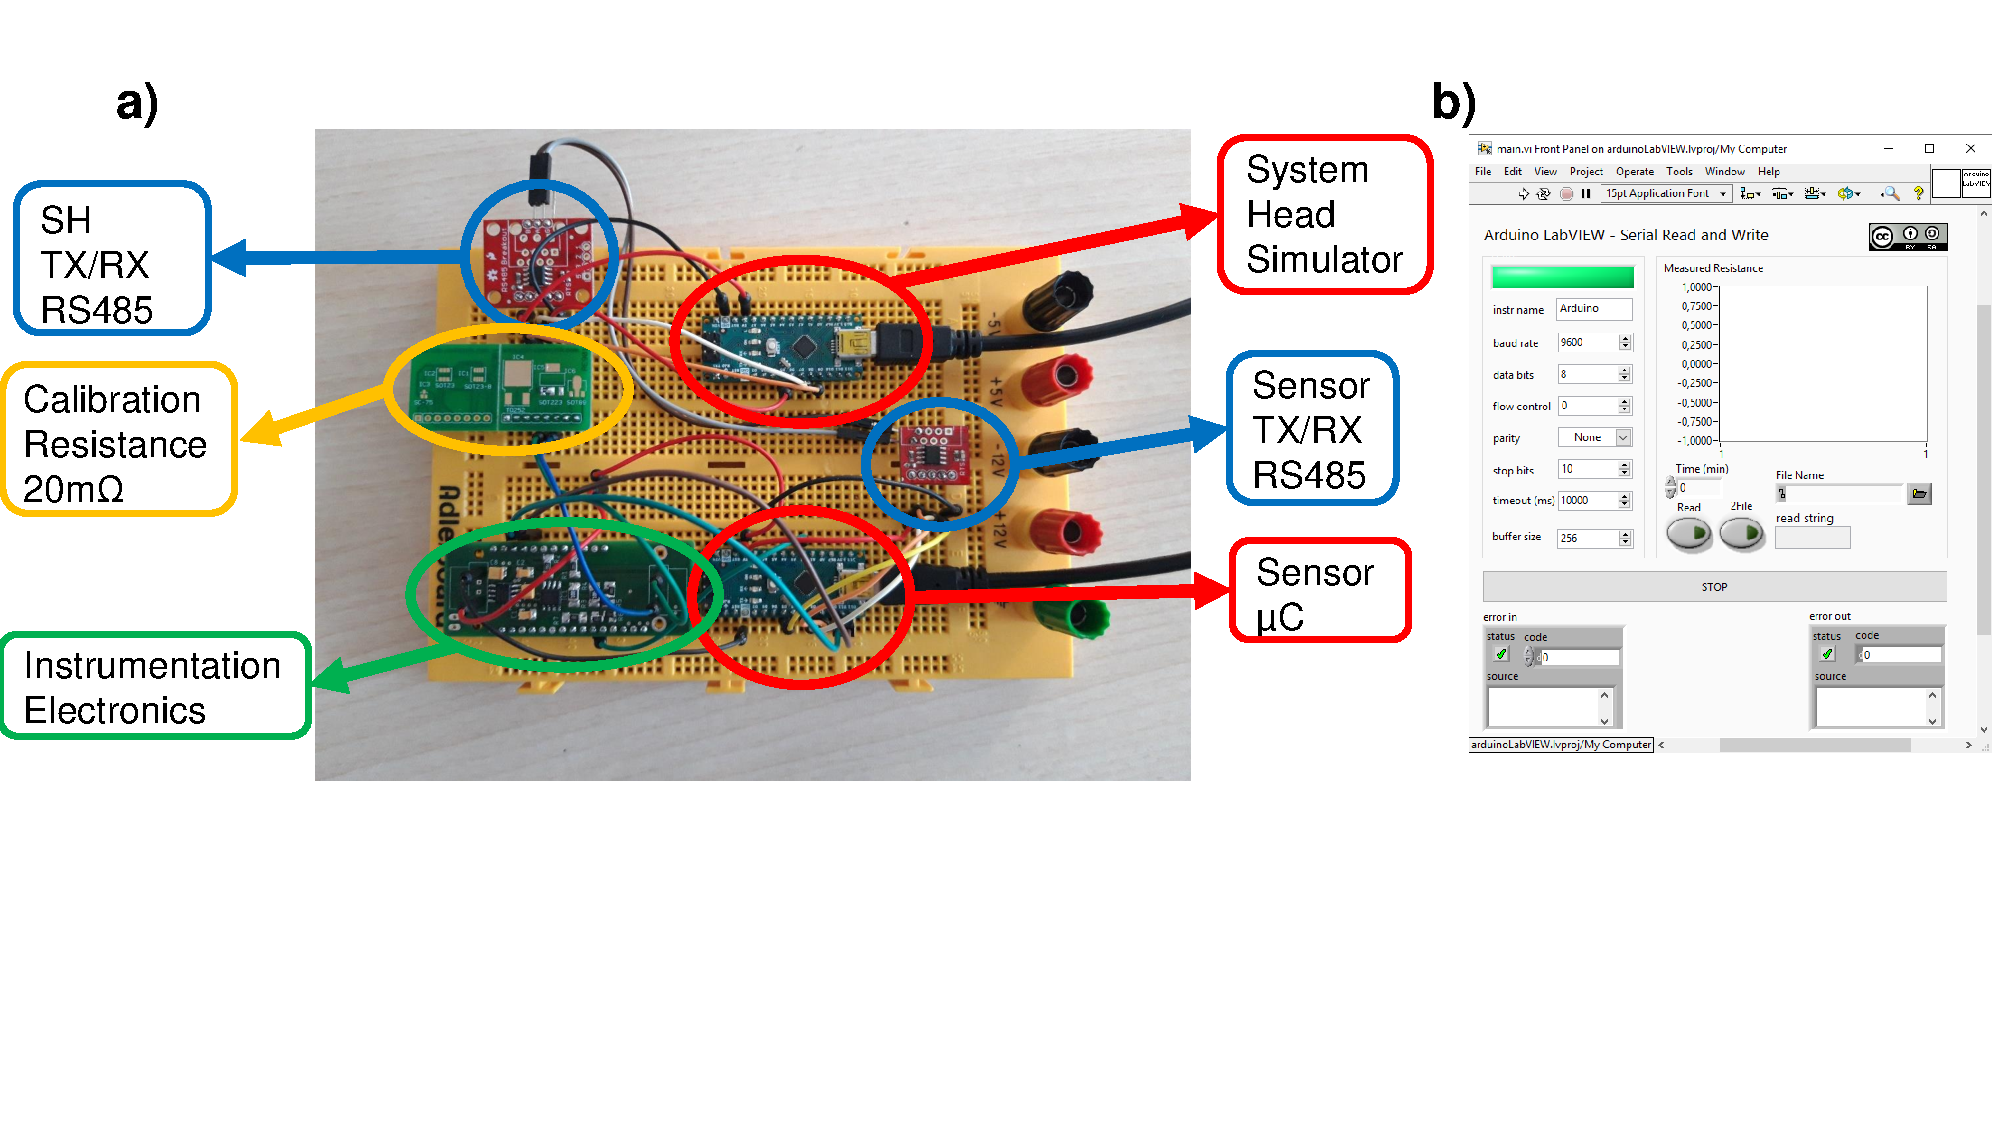
\includegraphics [trim = 0mm 50mm 0mm 0mm, clip, width=1\textwidth]{images/fig4.pdf}
%\hfill
\caption{Experimental Setup assembled for calibration and test purposes. (a) Hardware includes the SP3485 interface of the sensor, instrumentation electronics and the $\mu$C in charge of measurements and a control resistance of $20$\,m$\Omega$. It also incluse an extra SP3485 interface and ARDUINO Nano which simulates the System Head asking for measurement and collecting data. (b) The $\mu$C simulating the System Head is controlled by a PC via LabVIEW application running in a stand alone PC. The application sends an ASCII character to the $\mu$C in the sensor and waits for the resistance measurement. Once the data has arrived, the application stores it in a designated .txt file.}
\label{fig:measSet}
\end{figure*}
The System Head is simulated using an ARDUINO Nano controlled by a LabVIEW application running in a standalone PC. The application sends a serial command to the ARDUINO Nano which translates to an ASCII character and sent through the RS485 interface. Whenever the sensor RS485 interface passes the character to its $\mu$C, the measurement starts using the instrumentation electronics. A $20$\,m$\omega$ resistor was attached to the electronics for calibration purposes. The total resistance of the current path was measured with a 34401A digital multimeter from KEYSIGHT, being $51.3$\,m$\Omega$ on average, which is still in the range of the Ohm-meter (maximum resistance of $70.779$\,m$\Omega$).

This prototype was modified in order to perform measures of the sensitive body inside a solution of \textit{Aqua Regia} and deionized water in different concentrations. This was intended to accelerate the corrosion phenomena, allowing to register data and calibrate the electronics. %Figure~\ref{fig:measSet_2} shows t%
The instrumentation electronics were placed in a suitable platform and connected to a Power\,$\&$\,Communications line heading to the RS485 interface in the simulated system head. The simulated System Head remained built on the prototyping board shown in figure~\ref{fig:measSet}. This version of the laboratory prototype was the basis of the Field Prototype presented in section~\ref{ssec:fieldProto}.
%\begin{figure}[!b]
%\centering
%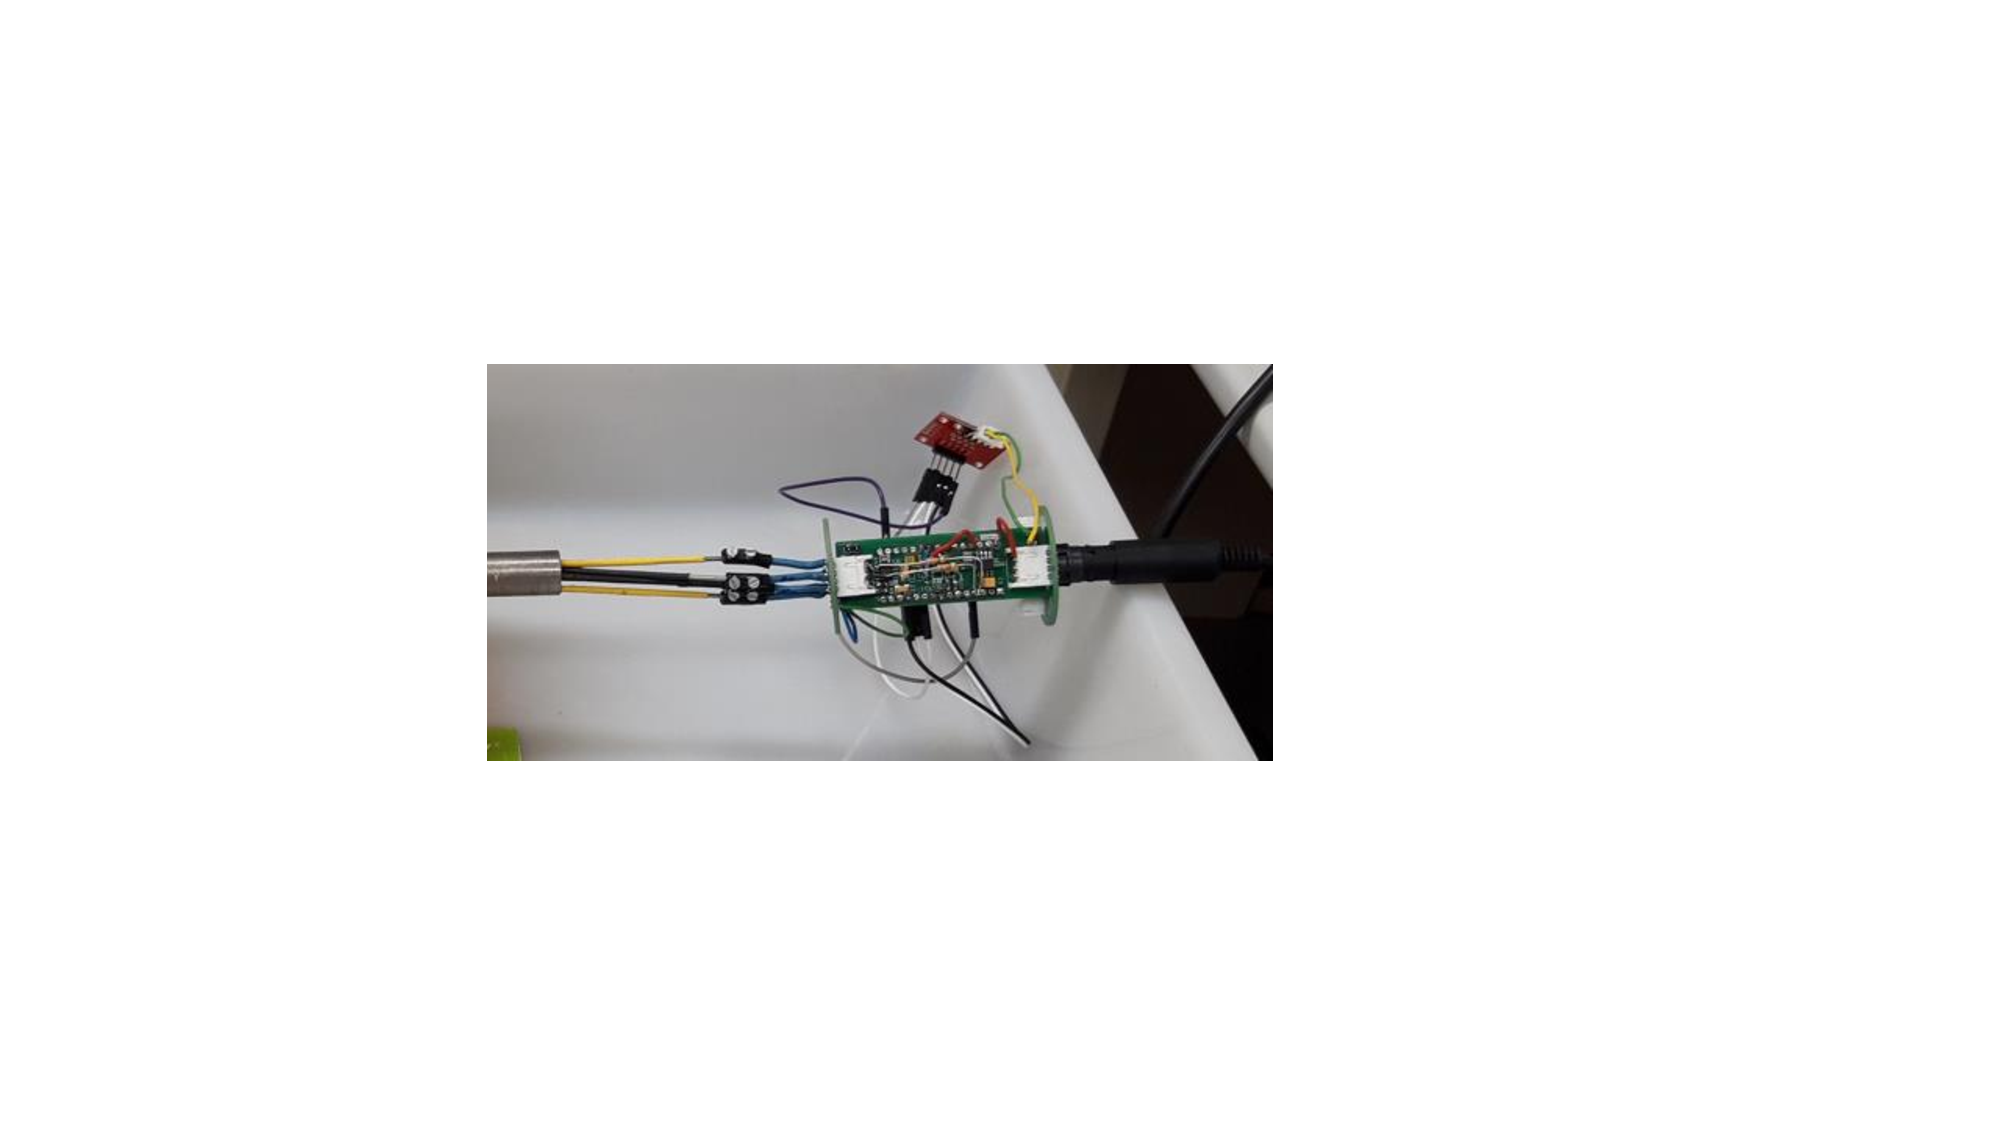
\includegraphics [trim = 80mm 70mm 120mm 70mm, clip, width=1\columnwidth]{images/fig5.pdf}
%\hfill
%\caption{Modified version of the laboratory prototype. The electronics and the $\mu$C were placed in a suitable FR4 PCB platform and connected to the sensitive body (left hand of the picture) via support PCB plus $4$ AWG$12$ wires. Communications and power were provided to the electronics via a $4$ cores shielded wire plus connector (right hand of the picture).}
%\label{fig:measSet_2}
%\end{figure}

\subsection{Field Prototype}
\label{ssec:fieldProto}
% Description of the measurement system 
\begin{figure}[!t]
\centering
\subfigure{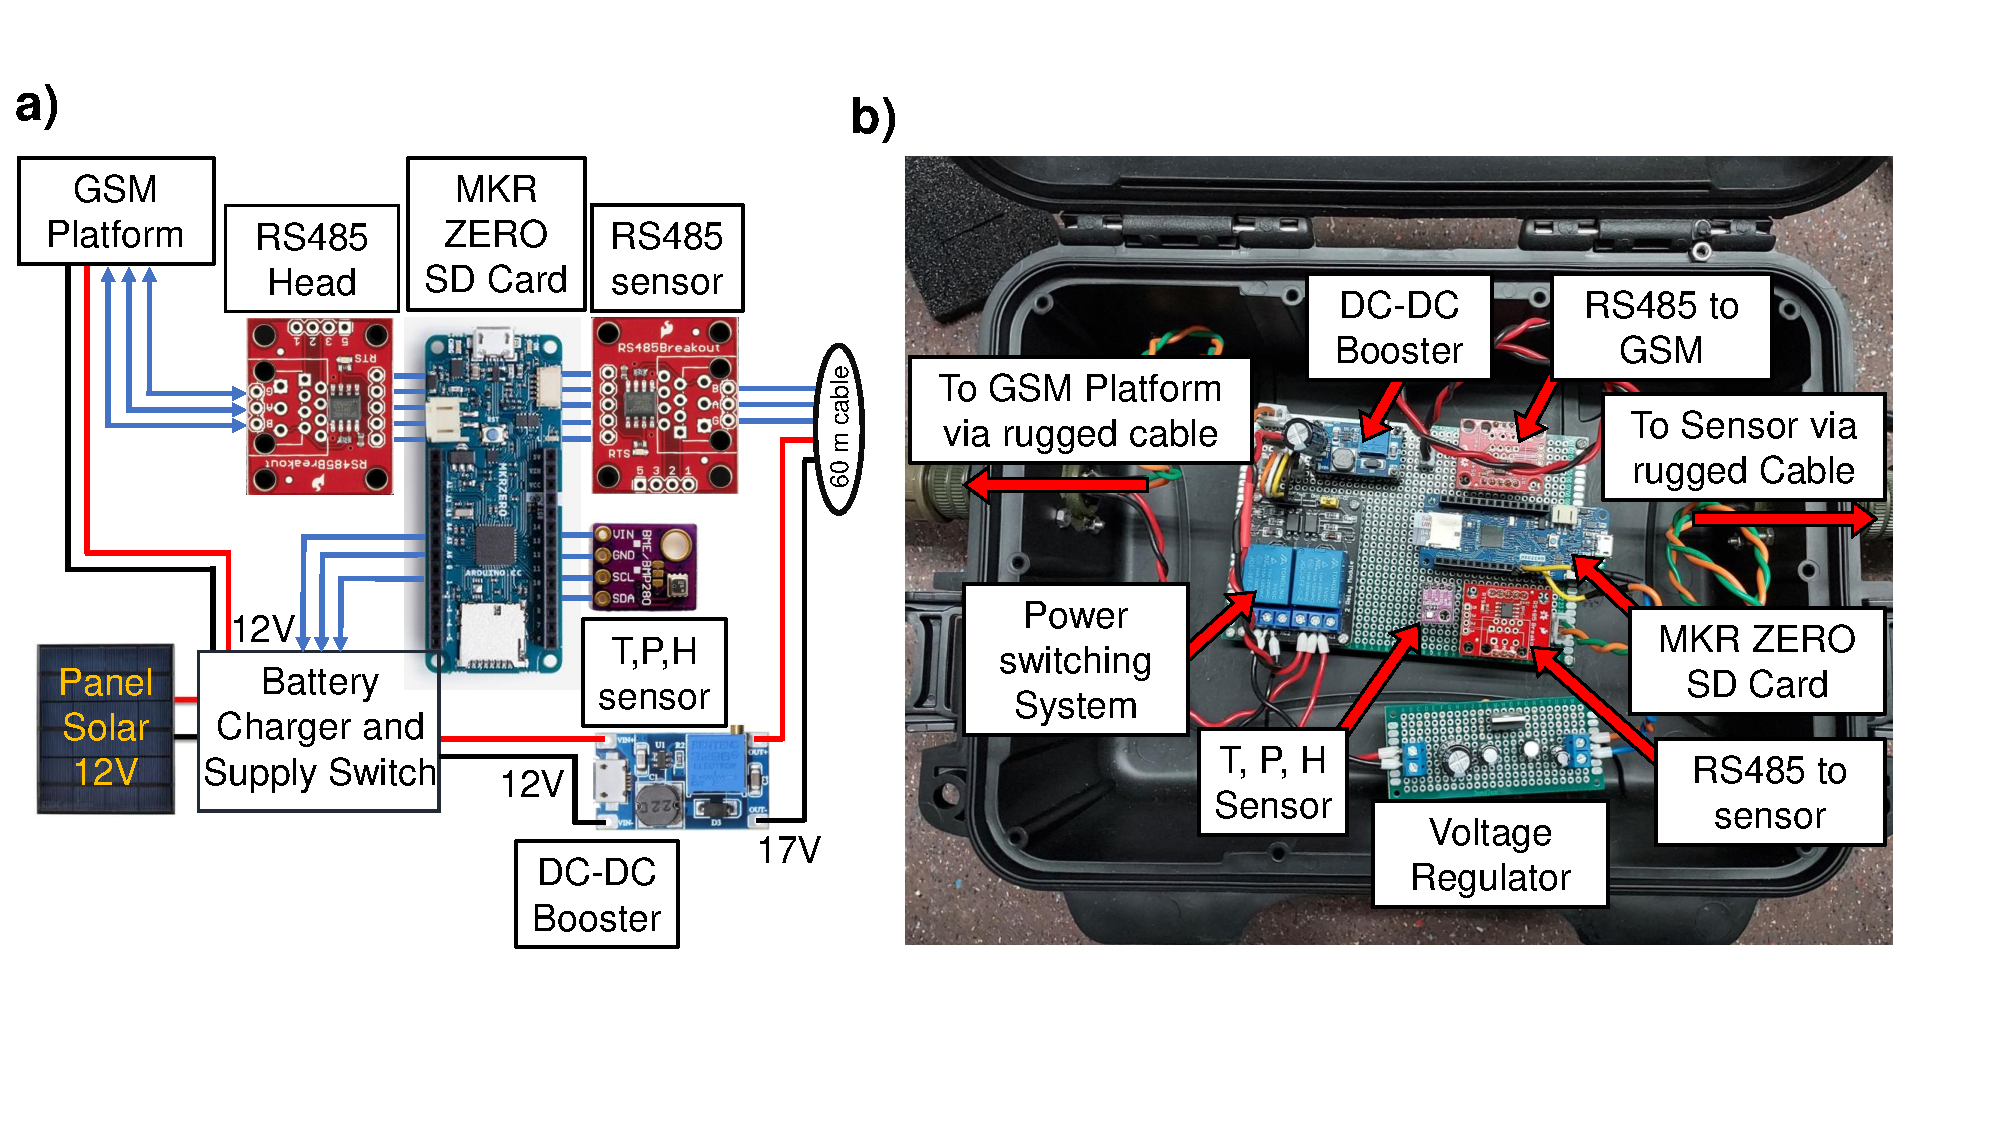
\includegraphics [trim = 0mm 30mm 0mm 0mm, clip, width=1\columnwidth]{images/fig6_v2.pdf}}
\subfigure{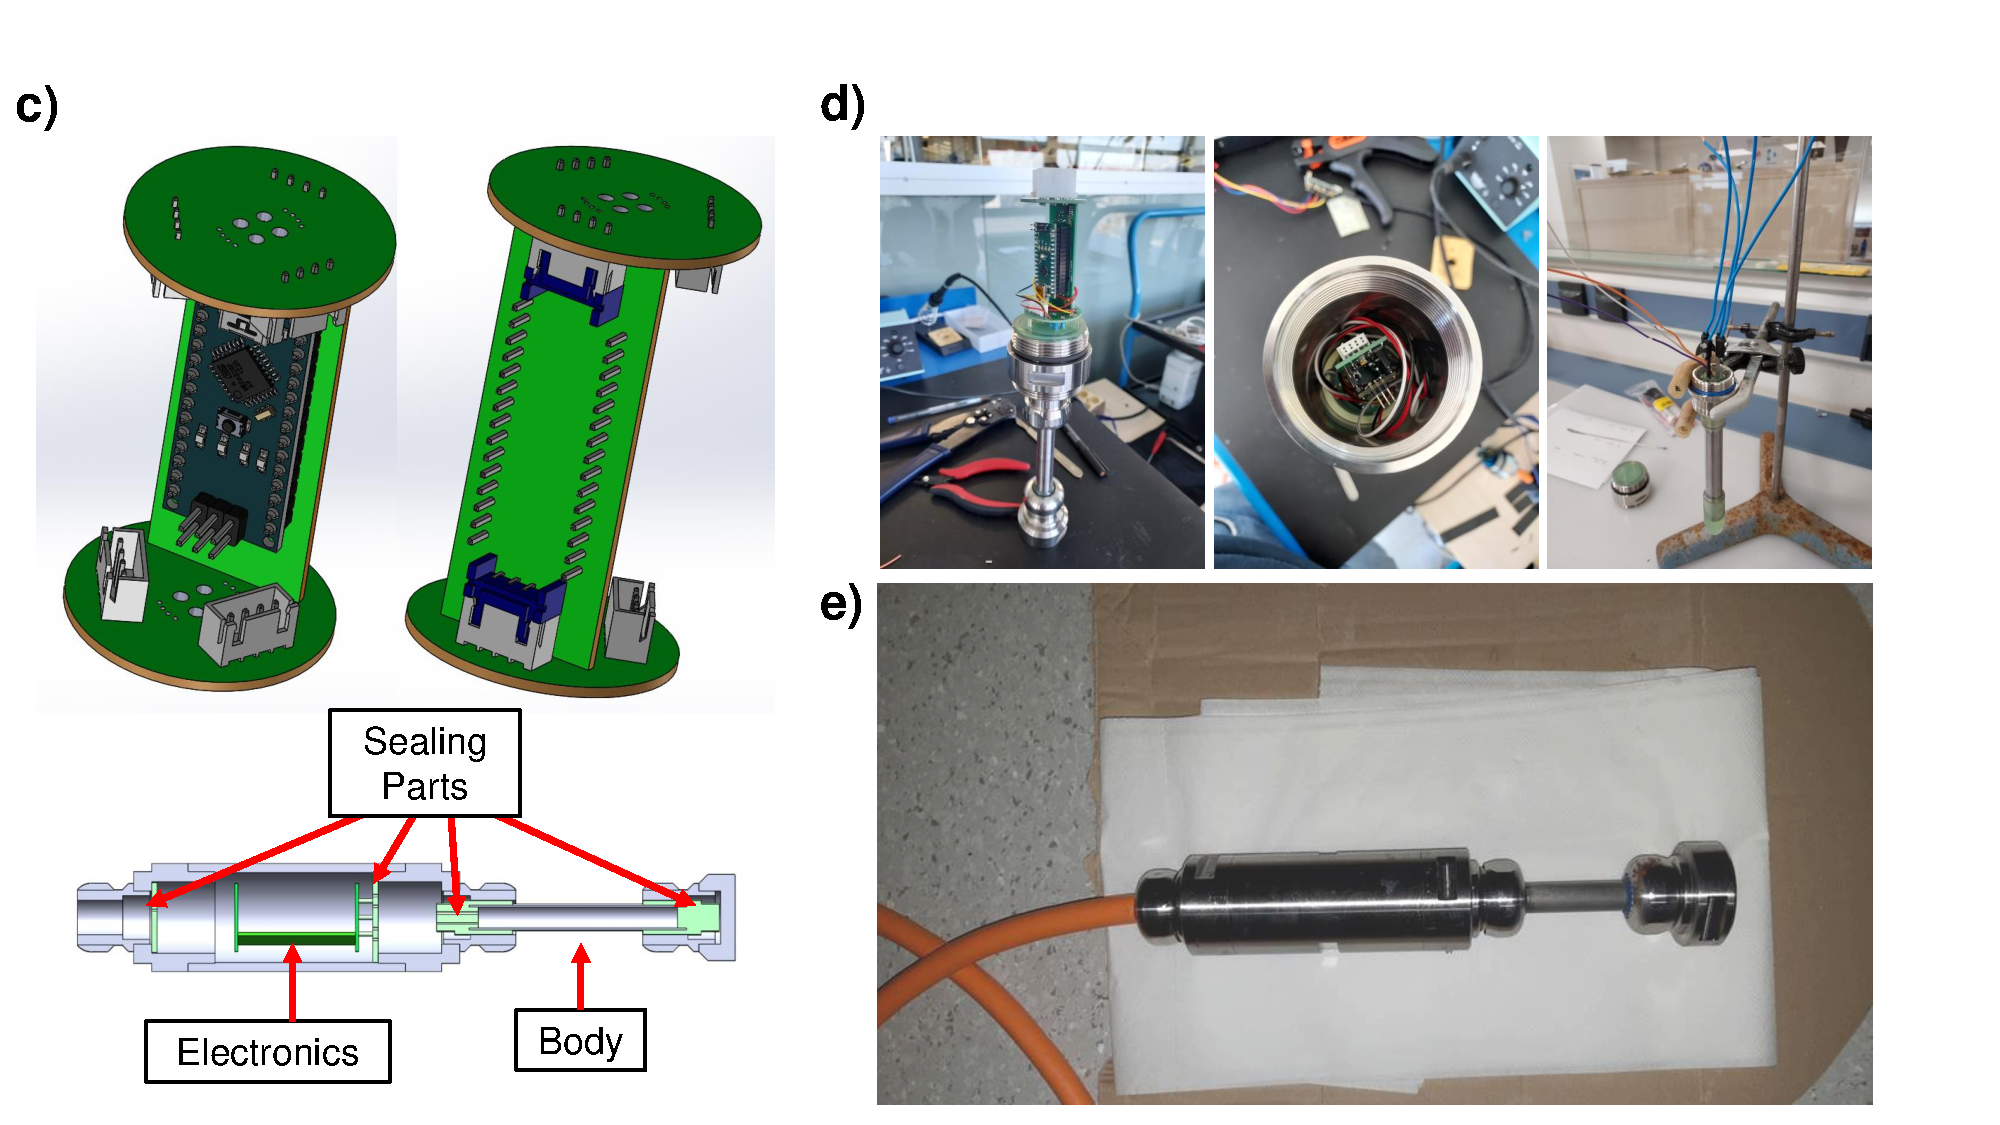
\includegraphics [trim = 0mm 0mm 0mm 0mm, clip, width=1\columnwidth]{images/fig6_2_v2.pdf}}
%\hfill
\caption{Field Prototype design diagrams and implementation. (a) Design diagram of the system head with an MKRZero controlling the measurement, GSM connection, data collection and power handling. (b) System Head implemented inside a rugged box with two military grade connectors towards the GSM platform and the sensor respectively. (c) Design diagrams of the sensor platform and the supports for the electronics. The body is grabbed by two cable glands and sealed by two 3D printed parts with holes for the connection bars. Electronics are placed inside a cylinder made of stainless steel and anodized to reduce fouling during operation. This cylinder is also sealed with 3D printed parts with holes for cable connections. Every cable connection is sealed with epoxy in order to ensure water tightness. (d) Implementation of the Field Prototype in different steps. (e) Sensor of the Field Prototype assembled and ready to use. The rugged cable is attached to the structure by a cable gland and the power and communications wires fixed to the top sealing 3D printed part with epoxy.}
\label{fig:measSet_3}
\end{figure}

Figure\,\ref{fig:measSet_3}\,(a) and (b) show the building plan and implementation of the System Head commanding the Field Prototype. The brain of the system is an MKRZero working as master and connected to the GSM platform and the sensor via two RS485 interfaces. The solar panel and the battery charger are placed outside the MKRZero box and the power relay is directly controlled by the MKRZero. A temperature, pressure and humidity sensor is placed inside the box in order to prevent breaks of tightness inside the box. The sensor reports directly to the MKRZero and the data are stored in the SD card at the same time than the data coming from the sensor.

Figures\,\ref{fig:measSet_3}\,(c) and (d) show the design diagrams and the implementation process of the sensor responsible for collecting data in the Field Prototype. The FR4 PCB platform for the instrumentation electronics and the $\mu$C used in the Laboratory Prototype was modified again in order to ensure the performance when the sensor is immersed. At the same, time the body is held by a stainless steel structure with two cable glands and connected to the electronics through 3D printed sealing parts. Similar sealing parts are added to the stainless steel cylinder where the electronics are placed. These parts ensure that no water comes into the structure when the sensor is immersed. A final visual of the sensor for the Field Prototype is depicted in figure\,\ref{fig:measSet_3}\,(e).

The Field Prototype was duplicated and placed in two different sites. First, in order to test tightness and performance one replica was placed in a pool (filled with artificial seawater) sited in Tecnalia Research\,$\&$\,Innovation facilities in Donostia (Spain). Second, the other replica was placed in a marine facility that Tecnalia runs in the Cantabrian Sea (HarshLab). Both replicas were running at the same time with different sampling time in order to observe and predict in the pool the behaviour of the Field Prototype in the sea.
\vspace{0.5cm}
\section{Resistance Measurement in Corrosive Environments}
\label{sec:resMeasCorrEnv}

\subsection{Test and Temperature Calibration}
\label{ssec:tempCalibration}
In order to test the accuracy and resolution of the implemented sensor, the resistance of a R5 grade HSLA steel tube of $150$\,mm length with $13$\,mm and $12$\,mm outer and inner diameter respectively was characterised.

First, the resistance was measured with a different procedure than the presented Ohm-meter at a certain temperature. The measurement was performed by passing $1$\,A current through the tube and pooling the voltage with the 34461A digital multimeter from KEYSIGHT described previously. The temperature of the tube was kept at $\sim$\,$25$\,$^{\circ}$ by applying a constant flow of air and this temperature was measured with an external data logger recording measures from a thermocouple type-K touching the tube. The current was also recorded by measuring the voltage on a $22$\,$\Omega$ ($50$\,W) with an extra digital multimeter. The measurement lasted for $1$ hour and voltages were recorded every $10$ minutes. The average resistance of the tube was $\sim$\,$1.06091\pm37\times10^{-6}$\,m$\Omega$.

A similar experiment was set up involving the Ohm-meter presented in previous sections. The system was measuring the resistance of the HSLA steel tube inserted in the sensor body depicted in figure\,\ref{fig:measSet_3}\,(c), (d) and (e). The electronics were sending data to the system head every $10$ minutes for $2$ hours. The temperature was kept to $25$\,$^{\circ}$C in the same way it was done for the previous experiment. The average value of the measured resistance was $1.06088$\,m$\Omega$ which resulted in an $\Delta$R$=30$\,$\mu\Omega$. The test in repeatability was performed three times and $\Delta$R was consistent with differences in the range of the uncertainty presented in section~\ref{ssec:errorRmeas}.

Second, the evolution of the tube resistance with temperature was evaluated in order to decouple the effect of temperature from the increase of resistance due to corrosion. As it is well known, the resistance of any piece of metal depends heavily on the temperature of the piece itself. Usually, the temperature dependence of the metal piece resistance is modelled by the following equation:
\begin{equation}
\label{eq:tempRx}
R(T) = R_{0}\times\left(1+\alpha \Delta T\right)
\end{equation}
where R(T) is the resistance of the piece at a certain temperature T, R$_{0}$ is the resistance of the piece at certain temperature of reference, T$_{0}$, and $\Delta T=T-T_{0}$ is the temperature deviation of the piece from T$_{0}$.

In order to derive the $\alpha$ coefficient, a measurement of the resistance of the tube when the temperature oscillates around $25$\,$^{\circ}$C was performed. The Field Prototype was placed in a climatic chamber (see figure\,\ref{fig:tempCal}\,(a)) and thermalized at $2$\,$^{\circ}$C for $1$\,hour. The temperature of the chamber and the sensitive body were recorded simultaneously. Once the sensitive body was at the environmental temperature ($21$\,$^{\circ}$C), the resistance was recorded during a program of $240$\,min where the temperature changed $0.16$\,$^{\circ}$C every minute.

Figure\,\ref{fig:tempCal}\,(b) shows the evolution of the resistance (in m$\Omega$) with T (in $^{\circ}$C). Disturbances between $12$ and $22$\,$^{\circ}$C were observed and only the relevant points are presented in the figure. These disturbances correspond to glitches in the power supply arriving to the electronics inside the sensor body. Despite the errors, a linear fit resulted in an $\alpha$ coefficient of $0.012 ^{\circ}$C$^{-1}$ with an R$^{2}=0.9755$. The uncertainty of this coefficient is similar to the uncertainty in the measurement of the resistance, $\sim$\,$\pm1.07\nicefrac{\mu\Omega}{^{\circ}K}$.

If the effects of corrosion and temperature are considered uncorrelated (as it is the case when the temperature is kept constant by the environment), the total resistance of the tube can be written as follows:
\begin{equation}
\label{eq:totalR}
R_{total} = R_{0}-\Delta R_{corr}+\Delta R_{T}
\end{equation}

where $\Delta$R$_{corr}$ is the increment of the resistance due to corrosion and $\Delta$R$_{T}=R_{0}\times\alpha\Delta T$ is the increment of the resistance due to temperature variations.
With this value, equations~\ref{eq:tempRx} and~\ref{eq:totalR}  can be rearranged as follows:
\begin{equation}
\label{eq:realRx}
R_{corr} = R(T)-R_{0}\times\alpha \Delta T
\end{equation}
considering always T$_{0}=25$\,$^{\circ}$C and monitoring the temperature of the tube at the same time, its resistance changes due to corrosion can be separated from temperature main influence, as intended.

\begin{figure}[!t]
%\centering
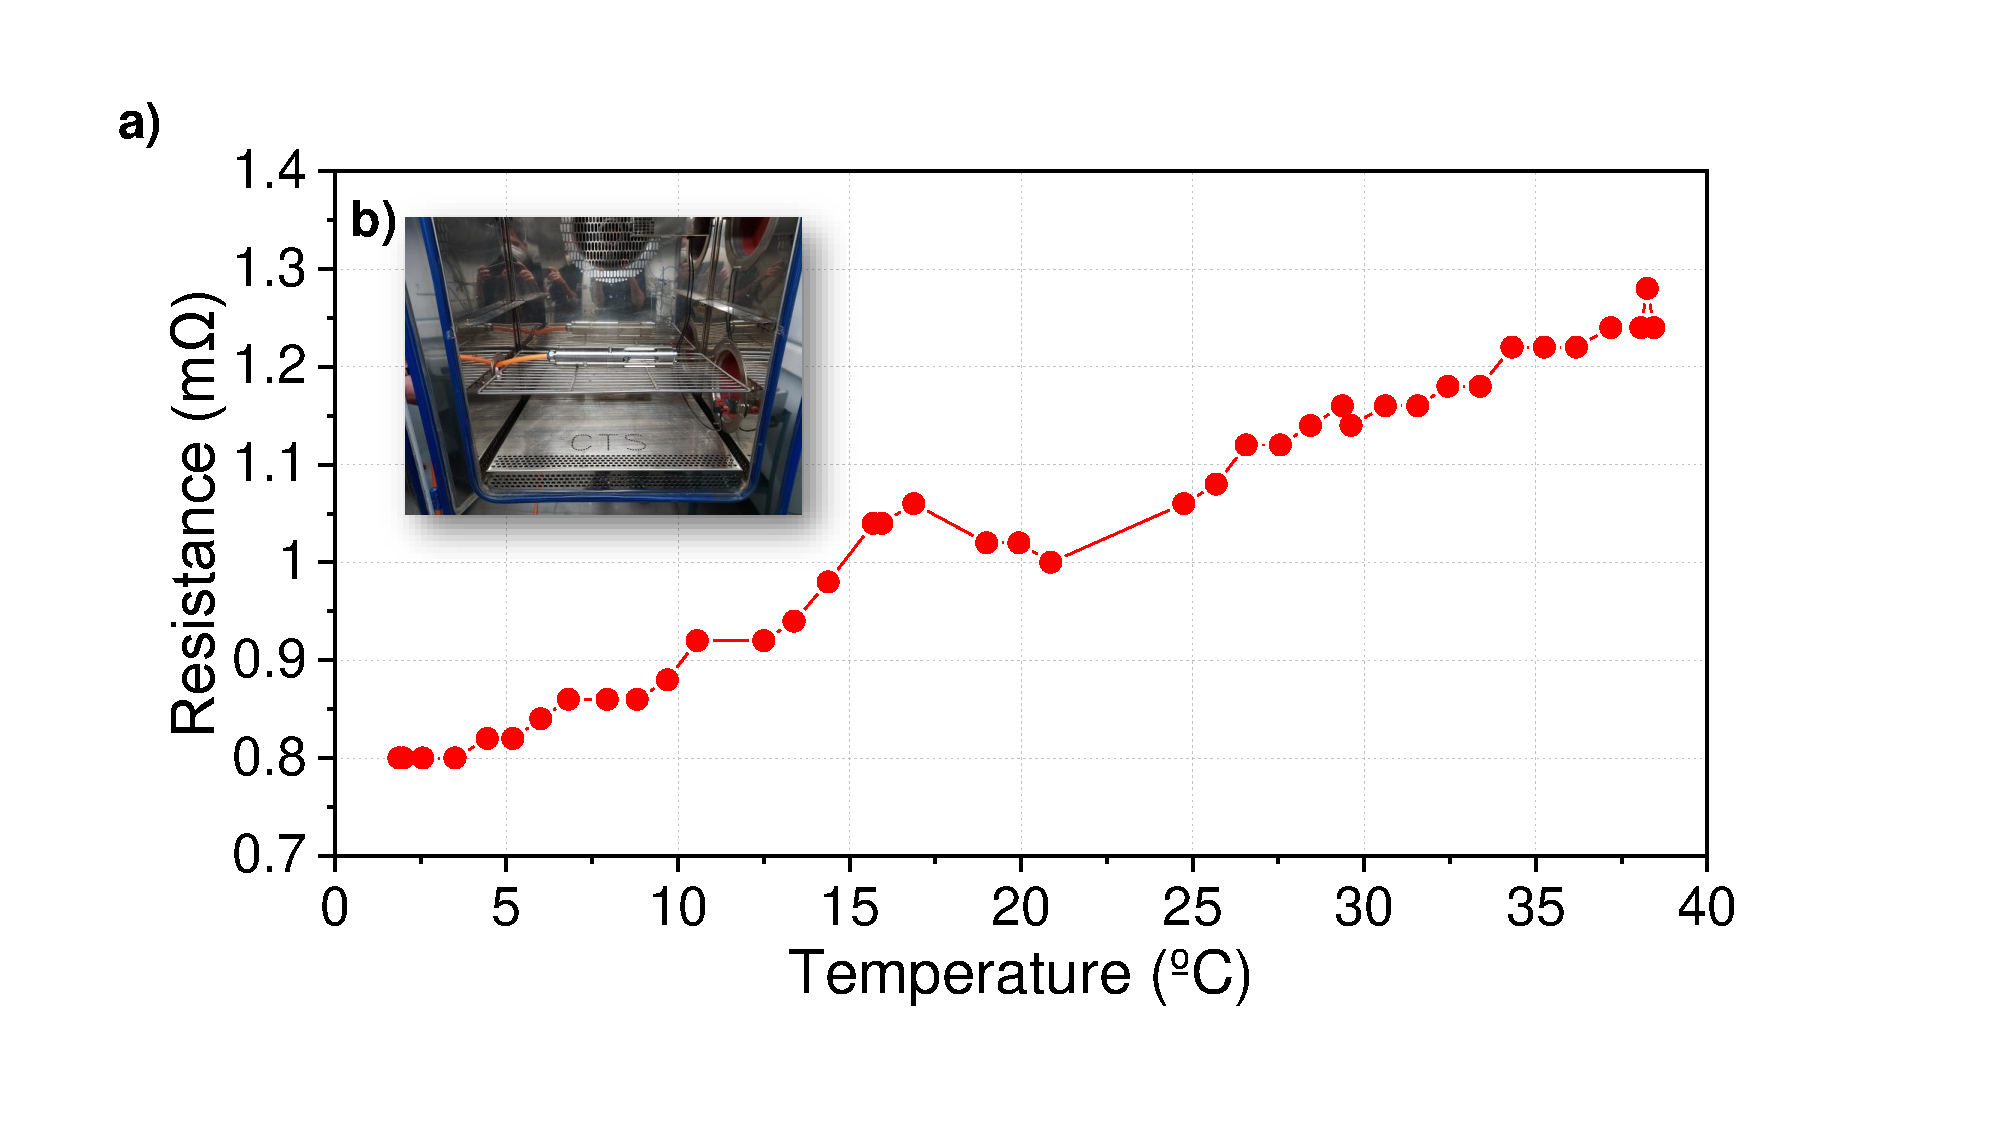
\includegraphics [trim = 20mm 20mm 35mm 12mm, clip, width=1\columnwidth]{images/fig7_v4.pdf}
%\hfill
\caption{Temperature calibration of the HSLA steel tube. (a) Evolution of the resistance (in m$\Omega$) with temperature measured with the electronics developed in this work. The measured resistance at $25$\,$^{\circ}$C was $1.060896$\,m$\Omega$ and the $\alpha$ coefficient was $0.012 ^{\circ}$C$^{-1}$ with a R$^{2}=0.9755$ obtained with linear curve fitting tools. (b) Prototype of the sensor body inside the climatic chamber. The temperature profile goes from $2$\,$^{\circ}$C to $40$\,$^{\circ}$C in $240$ minutes which results in temperature changes of $0.16$\,$^{\circ}$C. Samples of the resistance were recorded every 6 minutes, resulting in 40 samples.}
\label{fig:tempCal}
\end{figure}
%Error analysis and confidence interval estimation
\subsection{Measurements in \textit{Aqua Regia}}
\label{ssec:measAquaRegia}
In order to test the calibration performed in the previous section, a corrosion experiment was performed in \textit{Aqua Regia} (HNO$_{3}+3$HCl).

Figure\,\ref{fig:aquaRegia}\,(a) shows an HSLA steel tube (mechanized with the same dimensions presented before)  inserted in a corrosion chamber filled with \textit{Aqua Regia} diluted in water at $50\%$ ($1$:$1$). The tube was attached to the Ohm-meter as explained in section~\ref{ssec:labProto} and the resistance of the tube is recorded by a serial port with the LabVIEW application showed in figure\,\ref{fig:measSet}\,(b). At the same time, the temperature of the tube was recorded by inserting a thermocouple type-K in the chamber. The thermocouple was connected to the KEYSIGHT digital multimeter recording samples at the same time that the LabVIEW application via serial monitor.

Before measuring the resistance of the tube with the prototype, an estimation of the corrosion rate of the HSLA steel immersed in \textit{Aqua Regia} was performed. Three samples of the studied steel were immersed in a $50$:$50$ mixture of HNO$_{3}+3$HCl and water. The samples were $2\times2\times2$\,cm and they were immersed during different times. S$_{1,2}$ and S$_{3}$ were left in the solution for $3.25$ to $3.5$ hours and $19$ hours respectively. The corrosion rate was estimated by measuring the mass loss due to corrosion and certain dependence with immersion time was observed. This dependence is related to the accumulation of corrosion residues around the sample during the edging process~\cite{cramer2003A}. The estimated corrosion rate, after linear fitting of the available data, resulted in $1.763$\,$\nicefrac{\mu m}{hour}$ for the t$_{0}$ corrosion rate and a corrosion time-dependence of $-0.069$\,$\nicefrac{\mu m}{hour}$. Despite the lack of data, the corrosion rate and time dependence agree with the results presented in established literature for carbon steel samples~\cite{cramer2003B}.

\begin{figure}[!t]
\centering
\subfigure{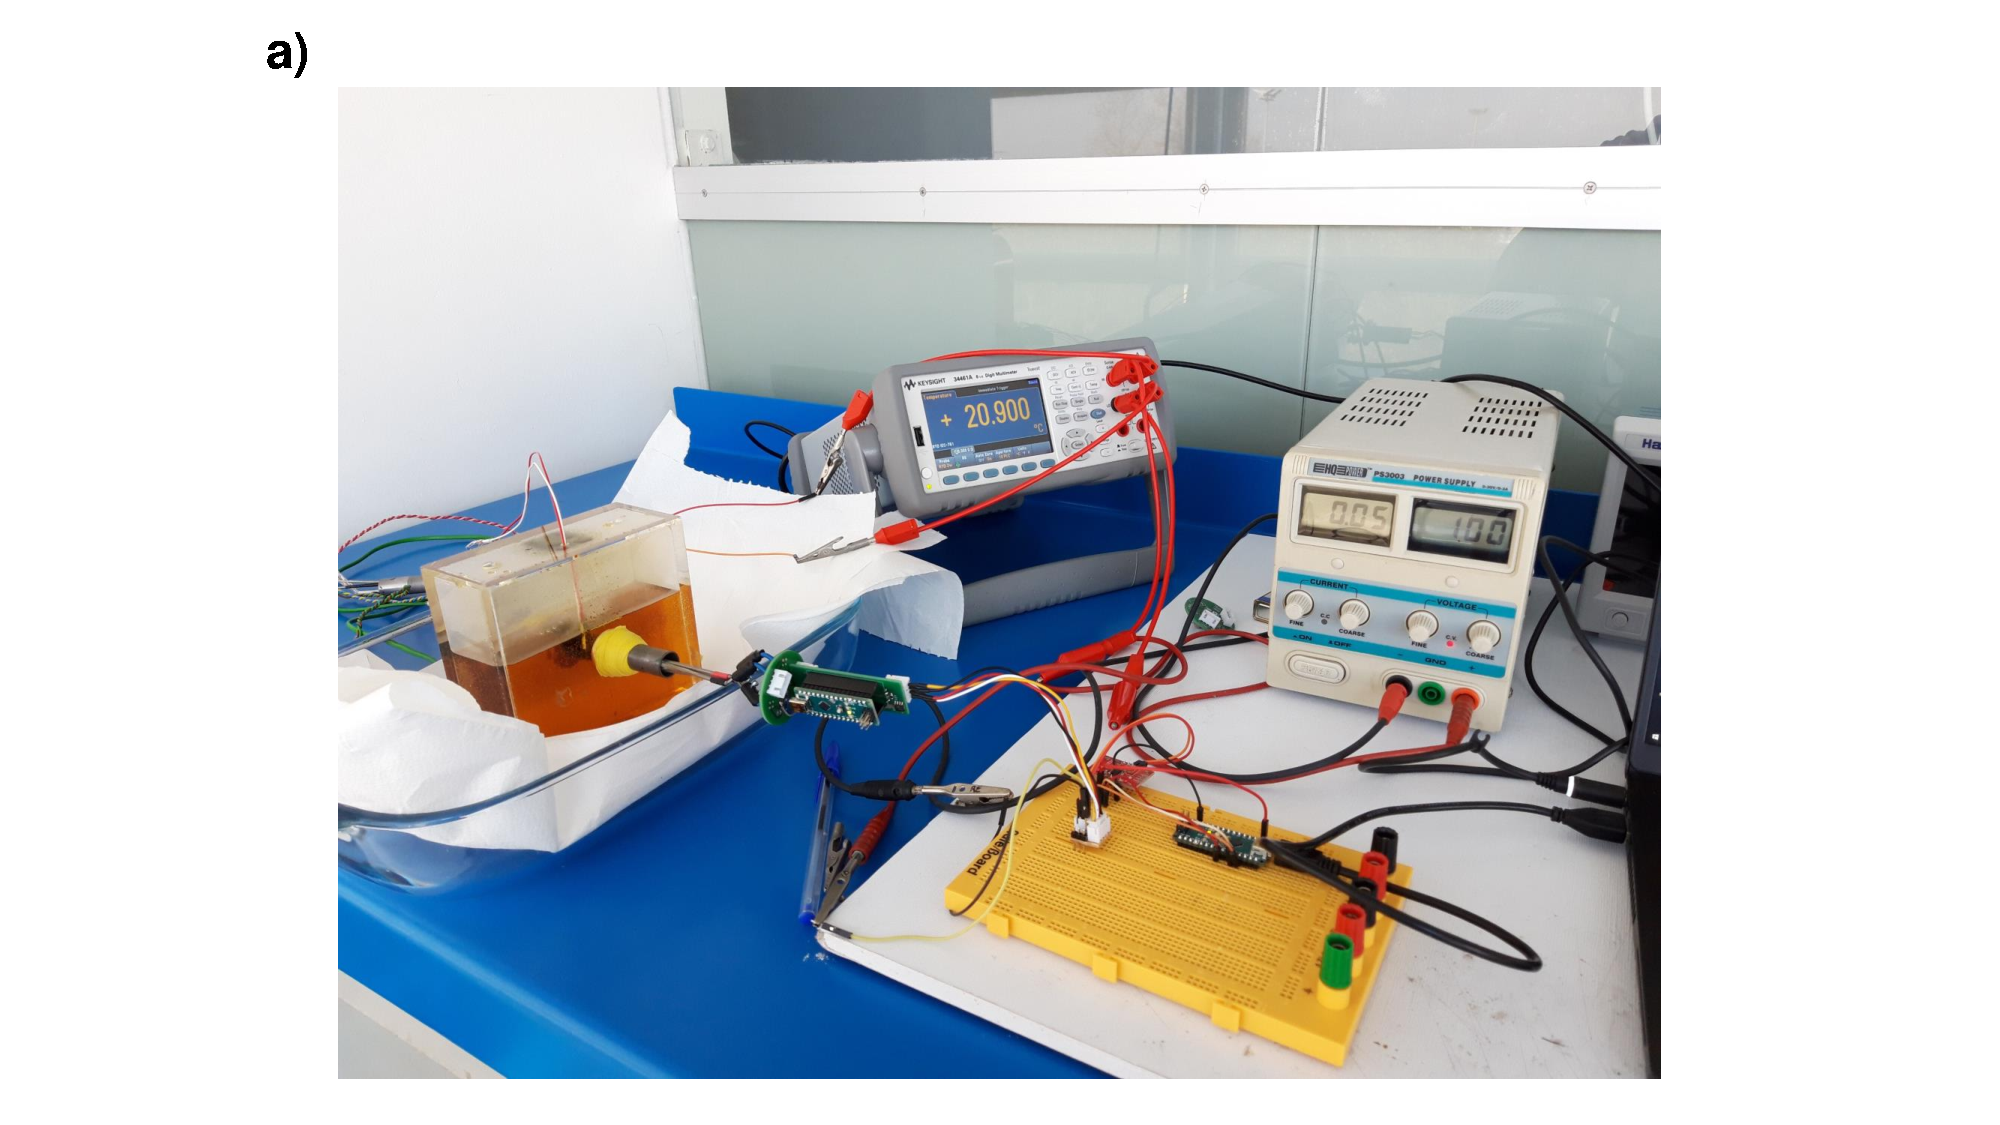
\includegraphics [trim = 40mm 0mm 40mm 0mm, clip, width=1\columnwidth]{images/fig8_1.pdf}}
\subfigure{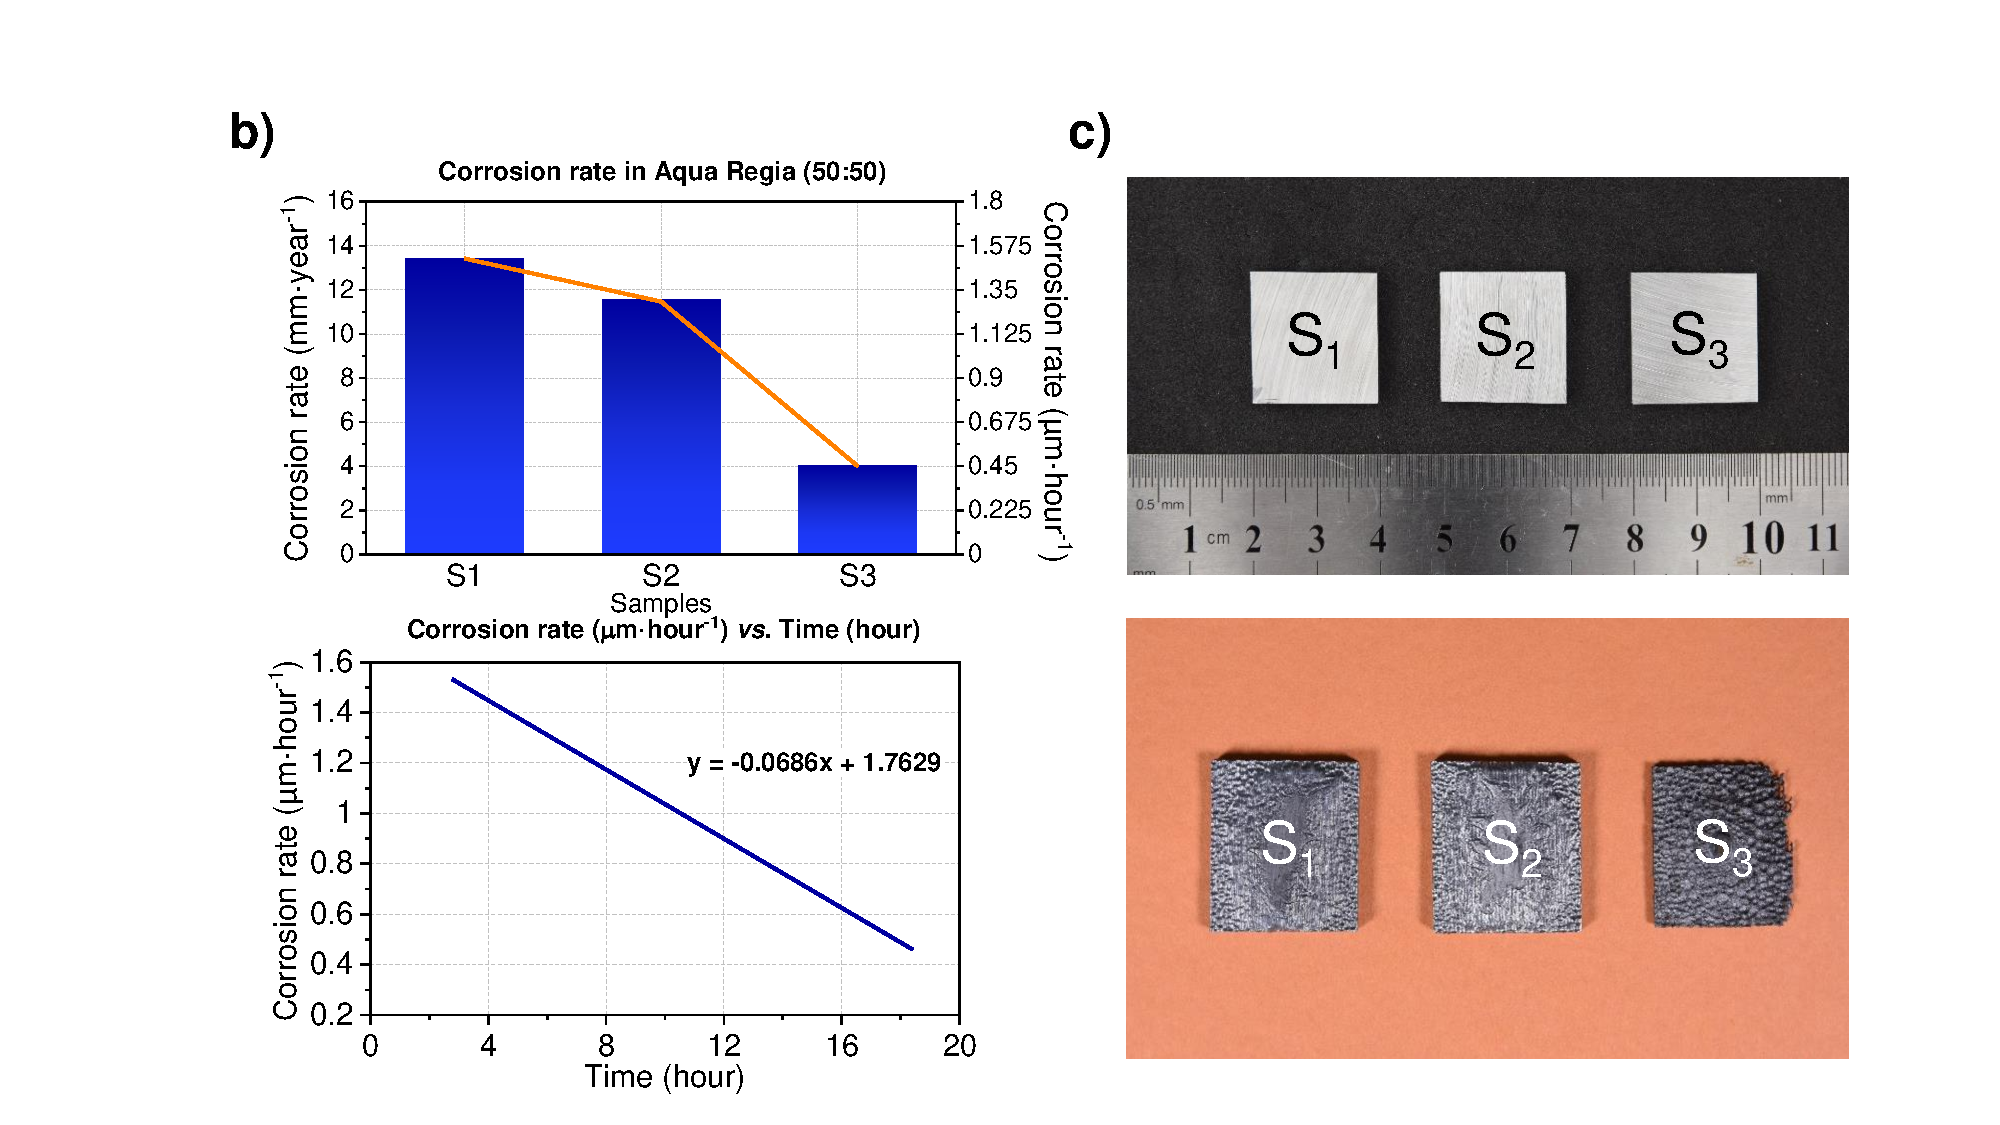
\includegraphics [trim = 40mm 0mm 20mm 20mm, clip, width=1\columnwidth]{images/fig8_2_v2.pdf}}
%\hfill
\caption{Measurement of the corrosion of a HSLA steel tube of $150$\,mm length and $13$\,mm and $12$\,mm outer and inner diameter respectively inserted in \textit{Aqua Regia} diluted in water at $50\%$. (a) Measurement setup based on the laboratory prototype presented in section~\ref{ssec:labProto}. The tube is connected to the Ohm-meter electronics as they are implemented in the Field prototype presented in section~\ref{ssec:fieldProto} but communicated with a System head simulator running in an ARDUINO NANO. The temperature of the tube is recorded by connecting a thermocouple type-K to a KEYSIGHT digital multimeter. (b) Measurement of the corrosion rate of HSLA steel samples immersed in \textit{Aqua Regia} diluted at $50\%$. S$_{1}$ and S$_{2}$ were immersed during $3.25$ to $3.5$ hours to test repeatability and S$_{3}$ was immersed during $19$ hours. The corrosion rate decreases with time due to the increasing width of corrosion products around the samples. (c) Pictures of the samples before and after immersion in the corrosive product. After $19$ hours the sample was almost destroyed.}
\label{fig:aquaRegia}
\end{figure}

Figure\,\ref{fig:aqRegiaResults} shows the recorded data during the experiment and the calculated R$_{corr}$. Measurements of the resistance were taken every minute for an hour. At the same the temperature was recorded as explained above. Figure\,\ref{fig:aqRegiaResults}\,(a) shows the evolution of both resistance and temperature values, with time. Peak values observed at minute $44$ were caused by the effect of localized corrosion on the tube. When corrosion residues were uniformly spread along the tube, the localized corrosion dominated in places where the dissolution had better contact with the surface. One of these spots was the place where the thermocouple touched the tube, causing galvanic corrosion. After two minutes, the spot was filled with residues and the recorded temperature came back to its normal pace.

$10$ minutes after the peak of temperature, the structural integrity of the tube was compromised. Pin-holes started to appear all over the tube and the measurement was corrupted.

\begin{figure}[!t]
\centering
\subfigure{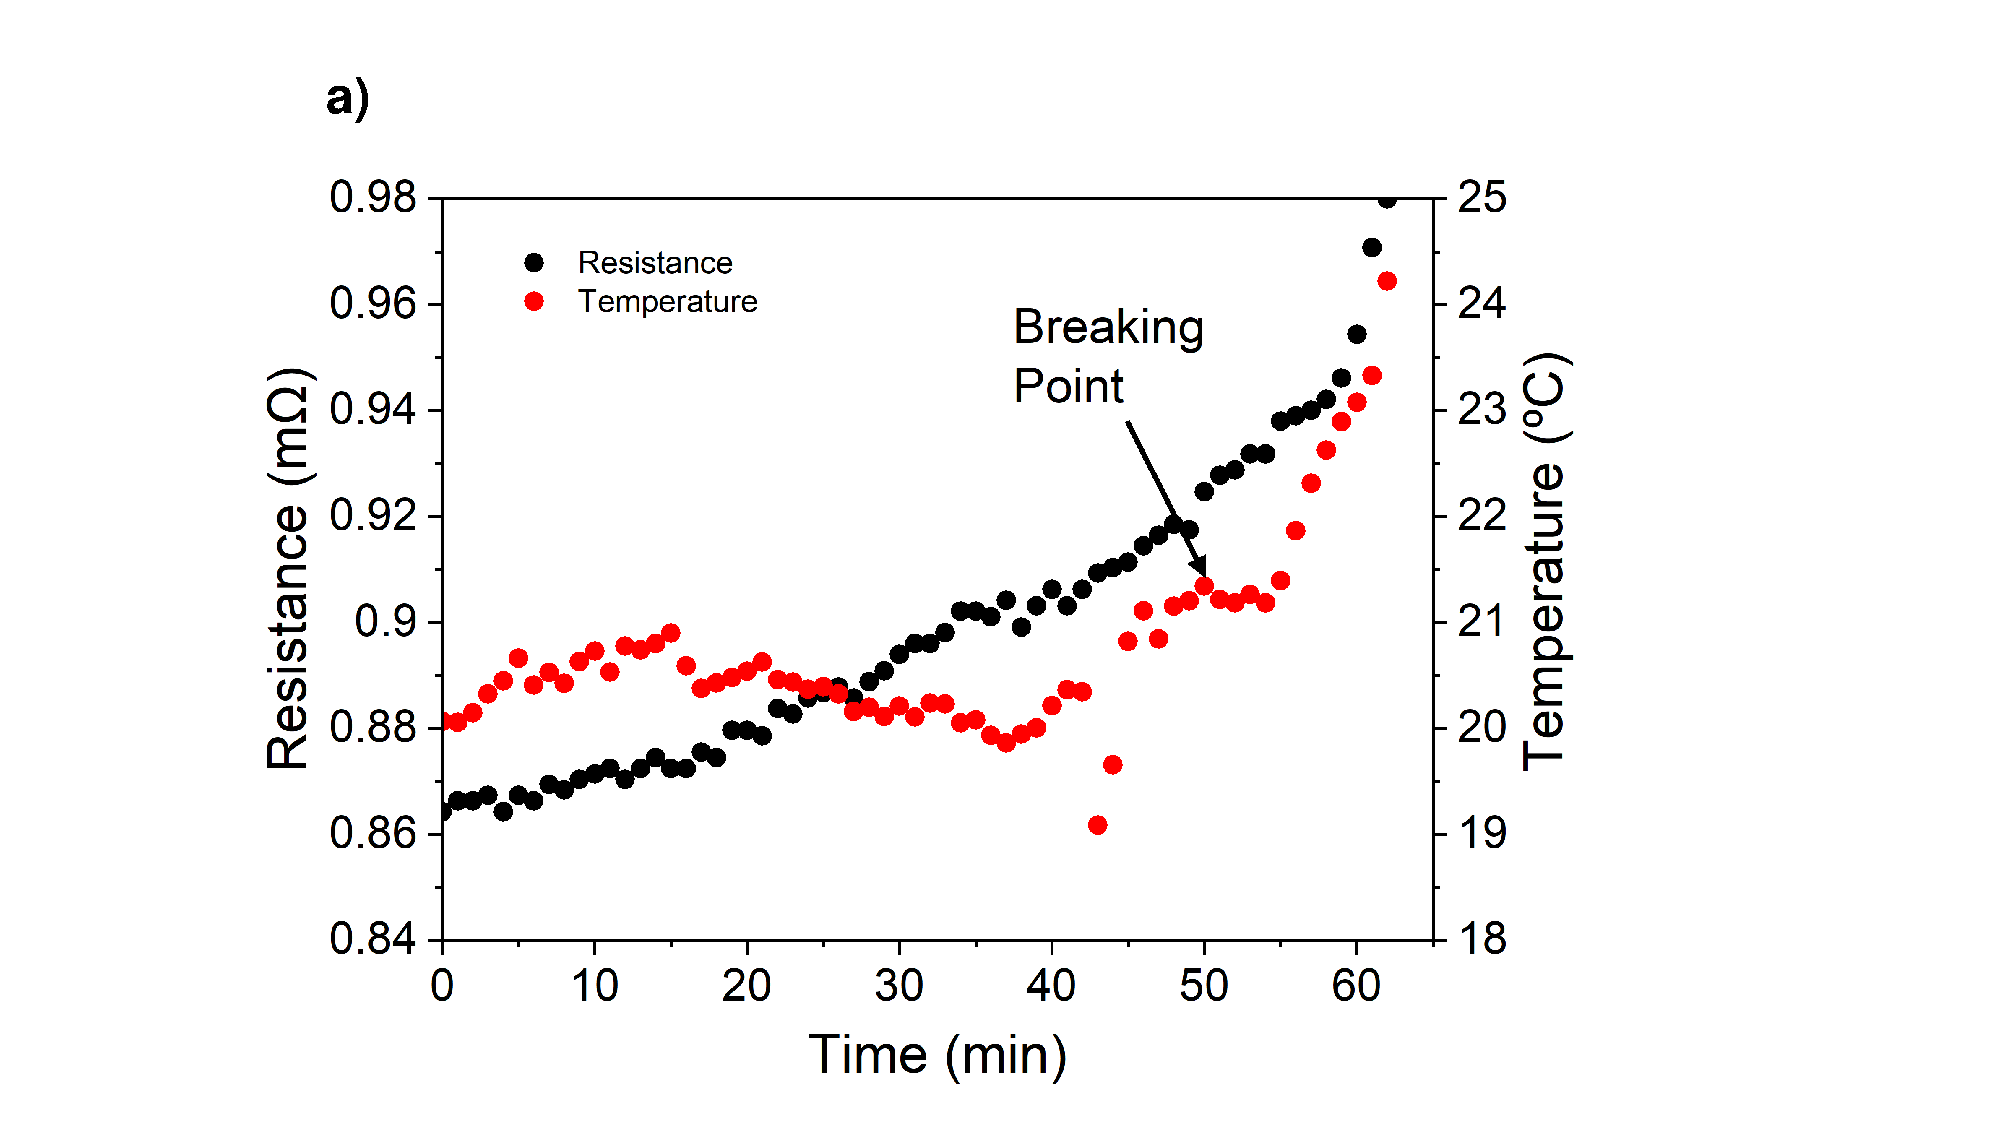
\includegraphics [trim = 40mm 0mm 70mm 0mm, clip, width=1\columnwidth]{images/fig9_1_v2.pdf}}
\subfigure{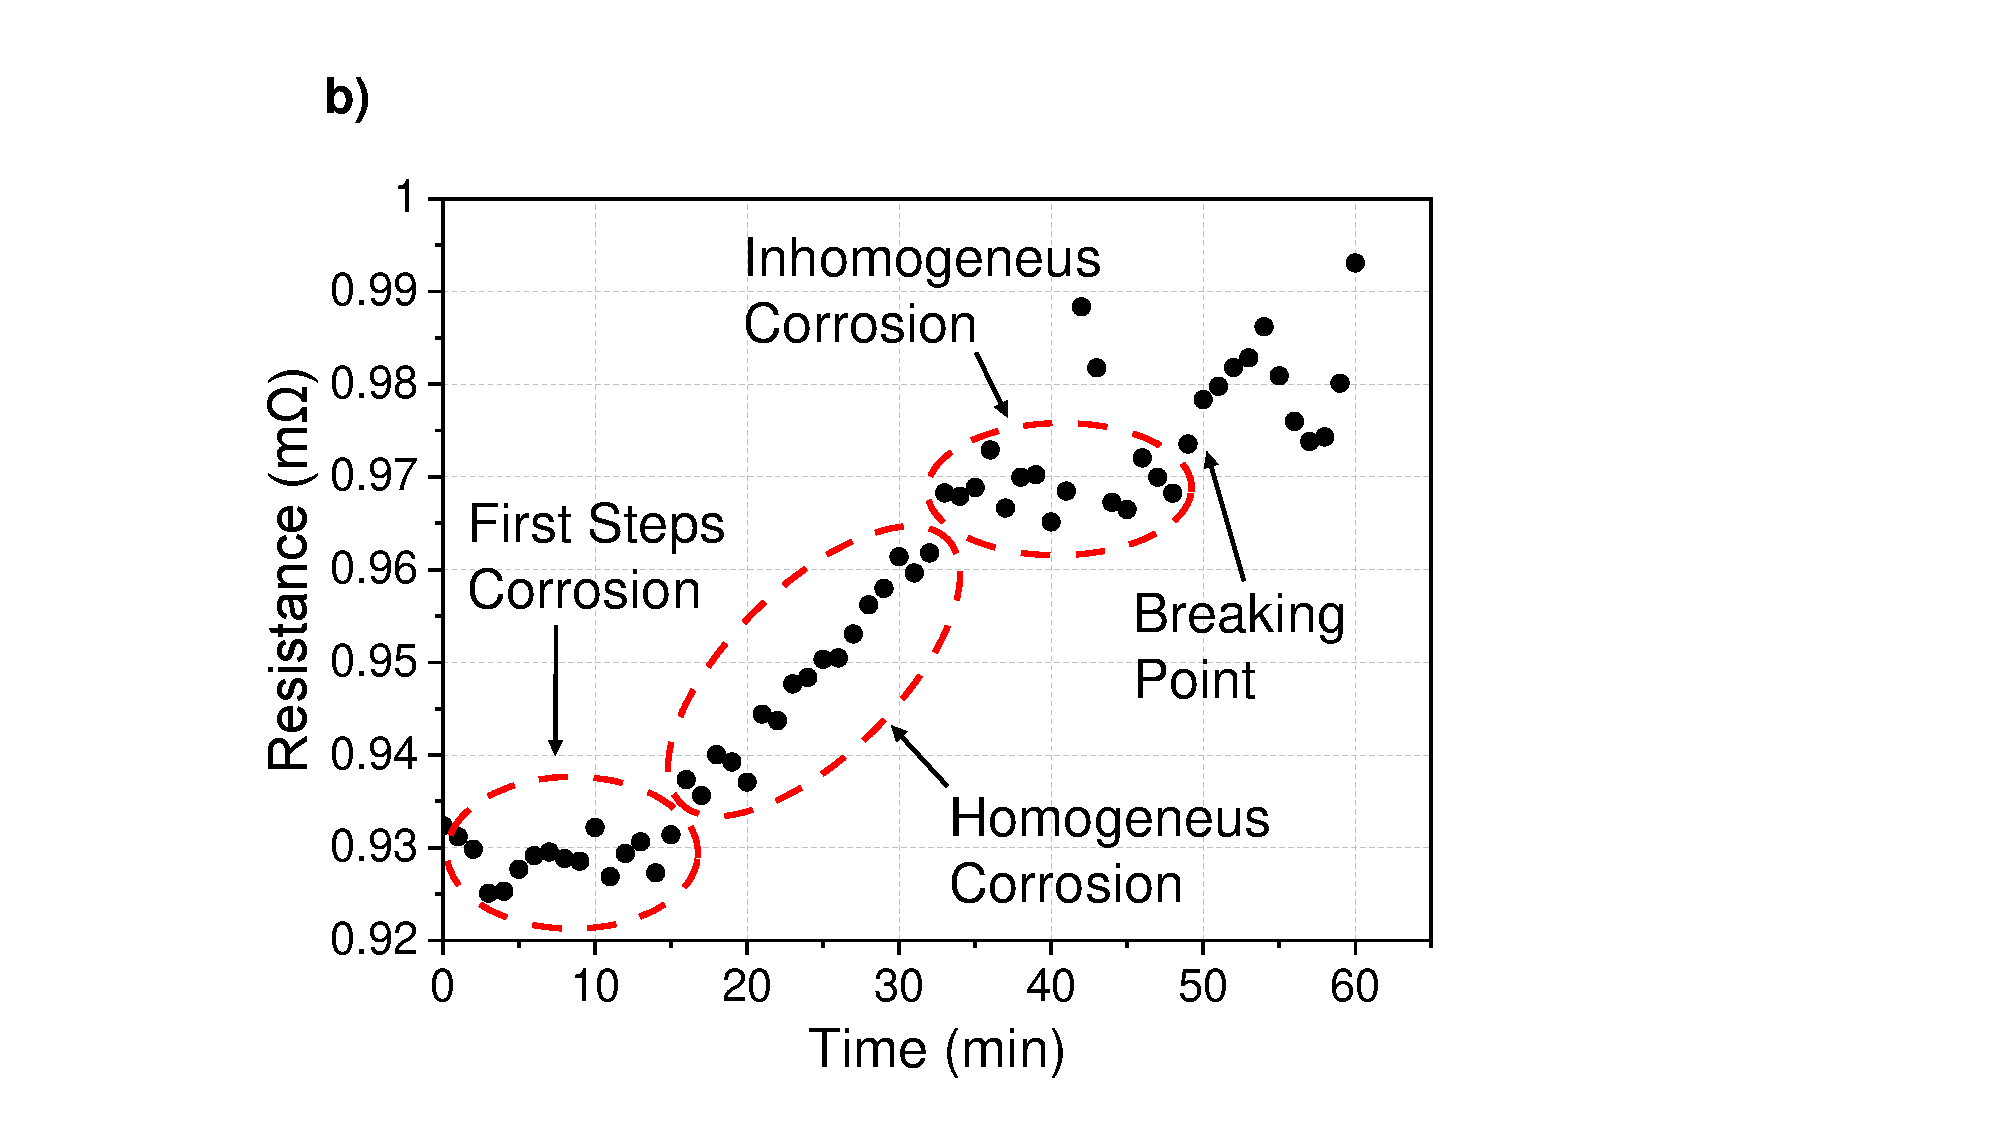
\includegraphics [trim = 40mm 0mm 70mm 10mm, clip, width=1\columnwidth]{images/fig9_2.pdf}}
%\hfill
\caption{Resistance and Temperature evolution of the R5 grade HSLA steel tube in a $50\%$ dissolution of HNO$_{3}$+$3$HCl in water. (a) Evolution of both variables with time. An abrupt change in temperature was observed at minute $44$ due to a localized corrosion effects. The tube presented holes at minute $51$ when localizaed corrosion started to dominated over homogeneous corrosion. (b) R$_{corr}$ calculated using equation~\ref{eq:realRx} where the temperature peak in minute $44$ is translated to an abrupt resistance change and evolution after the breaking point shows a high sensitivity to temperature.}
\label{fig:aqRegiaResults}
\end{figure} 

Figure\,\ref{fig:aqRegiaResults}\,(b) shows the resistance of the tube when equation~\ref{eq:realRx} is used on the resistance evolution depicted in figure\,\ref{fig:aqRegiaResults}\,(a). Three different corrosion phases were observed. First a slow-rate corrosion process was taking place. During the first 20 minutes, the polished surface of the tube stopped the corrosive ions of the dissolution from damaging the tube. In the following 20 minutes, a homogeneous corrosion process took place. The resistance increases linearly which can be understood as a generalized edging of the tube surface. At minute 36, the homogeneous process stops due to the appearance of inhomogeneous corrosion residues over the tube surface. The change in resistance decreases its speed before producing holes in the tube (around minute $51$).

The first two phases occur only at the beginning of the corrosion experiment (whenever the steel is immersed into the dissolution). Therefore, during long experiments, the corrosion rate in $\nicefrac{\mu\Omega}{hour}$ must be calculated from the data corresponding to T$=36$ to $51$. A linear fit of the points collected in this timeframe resulted in a corrosion rate of $0.2$\,$\nicefrac{\mu\Omega}{min}$ which corresponds to $\sim$\,$25$\,$\nicefrac{nm}{min}$. Therefore, the measured corrosion rate of the dissolution for the tube immersed is $\sim$\,$1.5\nicefrac{\mu m}{hour}$ which is relatively close to the result presented above for the arrangement depicted in figure~\ref{fig:aquaRegia}.
%Measurements and characterisation of the Seebeck effect.
\subsection{Measurements in Salt Water}
\label{ssec:measSaltWat}
Before immersing the sensor in a real offshore facility, it was placed in an \textit{inhouse} pool filled with artificial seawater at a concentration of $35$\,$\nicefrac{g}{L}$ as depicted in figure~\ref{fig:poolMeas}~(a). The sensor was connected to the System Head via a rugged cable (orange cable in the picture) of $\sim$\,$20$\,m long. At the same time, the System Head was connected to a Raspberry 4B (RPB4) acting as a GSM platform. The RPB4 received data from the System Head via RS485 interface and upload it to an internet dashboard based on GRAFANA.

The data upload to the dashboard consisted of the temperature of the tube after measurement, the temperature inside the sensor body containing electronics, the measured resistance of the tube and temperature, humidity and pressure inside the box containing the System Head. The data were uploaded and recorded in an SD card inside the System Head every $10$\,minutes.

Figure\,\ref{fig:poolMeas}\,(c) shows the measurements of temperature (\tikzbullet{red}{red}) and the resistance (\tikzbullet{black}{black}) of the tube for two days. The resistance values were corrected with equation~\ref{eq:realRx}. In order to test the temperature correction, the sensor was extracted from the pool for a period of time resulting in an increase of the temperature of $1.2$\,$^{\circ}$C due to manual handling of the sensor. After $490$ minutes the sensor was placed back into the pool. The corrected resistance shows no dependence on temperature, confirming the results obtained in section~\ref{ssec:tempCalibration}.

The measurements show a dispersion of $\pm0.03$\,$^{\circ}$C and $\pm2.05$\,$\mu\Omega$ for temperature and corrected resistance respectively. Therefore, the observable corrosion rate is $\sim$\,$0.46\,\nicefrac{\mu m}{yr}$ which is bigger than the uncertainty results presented in section~\ref{ssec:errorRmeas}. It has been experimentally probed that the ADC losses $1$-$1.5$\,bits whenever the power supply rails are not decoupled with suitable capacitors. The improvement of the sensitivity compared with commercial ER sensors does down to $\sim125$ for the best sensor presented in section~\ref{sec:intro}. At the same time, the evolution of the resistance shows fast changes (minute 2320 and 3210) with different implications. The first step (minute 2320), is related to the position of the sensor inside the pool. In the first place, the sensor was placed very close to the pool wall and the tube was in contact with some plastic parts of the pool. The position was corrected and the evolution changed to almost flat.

The second step is directly related with the extraction of the sensor out of the pool. During immersion and extraction of the sensor inside the salt water, it was observed that the resistance increased and decreased respectively. Although the phenomenon will be described thoroughly elsewhere, the theory of electrostatic explains the increase in resistance. Negative ions of the salt water gather around the steel tube whenever it is immersed in the dissolution in order to start the corrosion processes. As they gather, they produce an electric field surrounding the tube that pushes the electrons circulating through it to the tube inner surface.

The measurement inside the pool served as a control test of tightness, hardware performance and firmware reliability. The final prototype was taken to a Tecnalia facility at the Cantabrian Sea and placed as depicted in figure\,\ref{fig:poolMeas}\,(b).
\vspace{0.5cm}
\subsection{Measurements in the Cantabrian Sea}
\label{ssec:measCantSea}
\begin{figure}
\centering
\subfigure{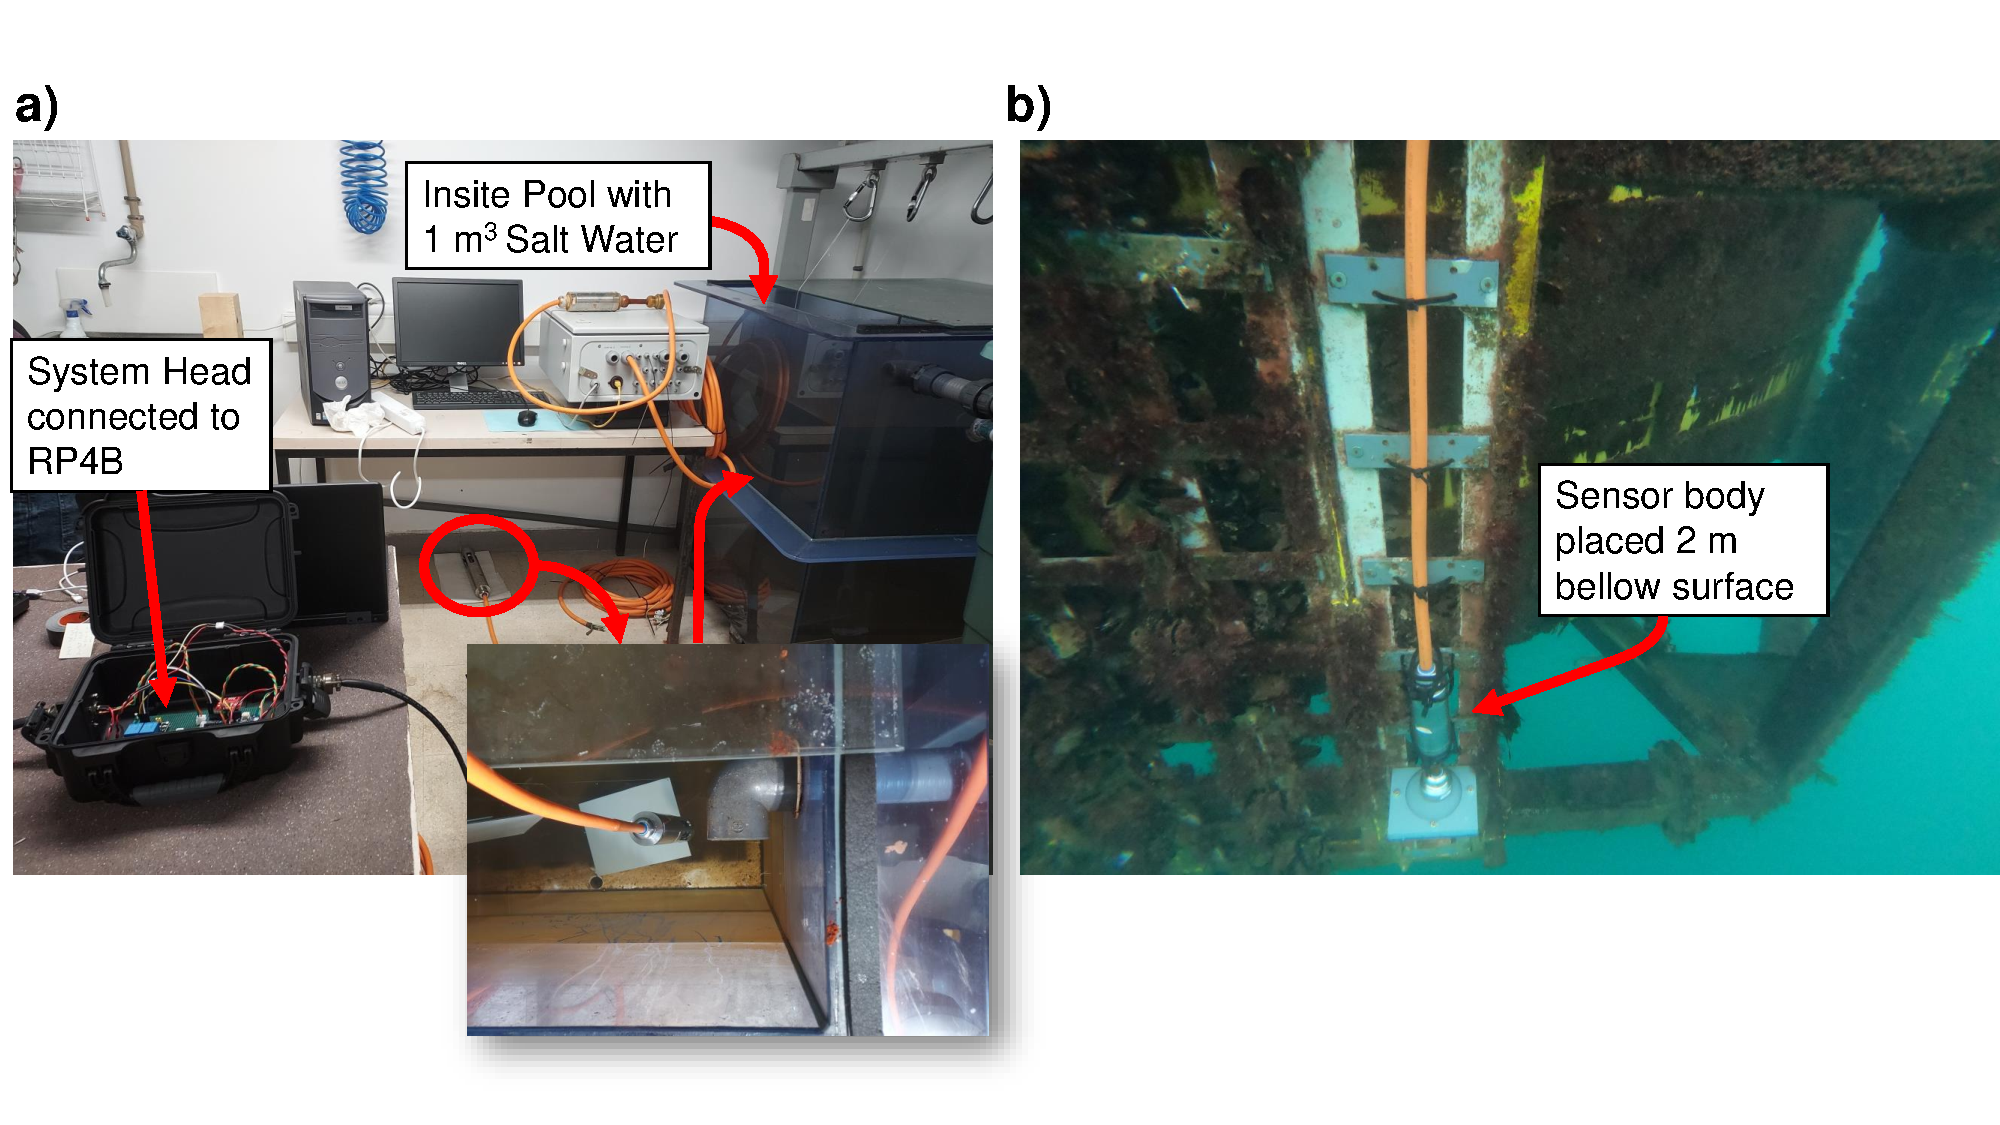
\includegraphics [trim = 0mm 0mm 20mm 10mm, clip, width=1\columnwidth]{images/fig10_1_v3.pdf}}
\subfigure{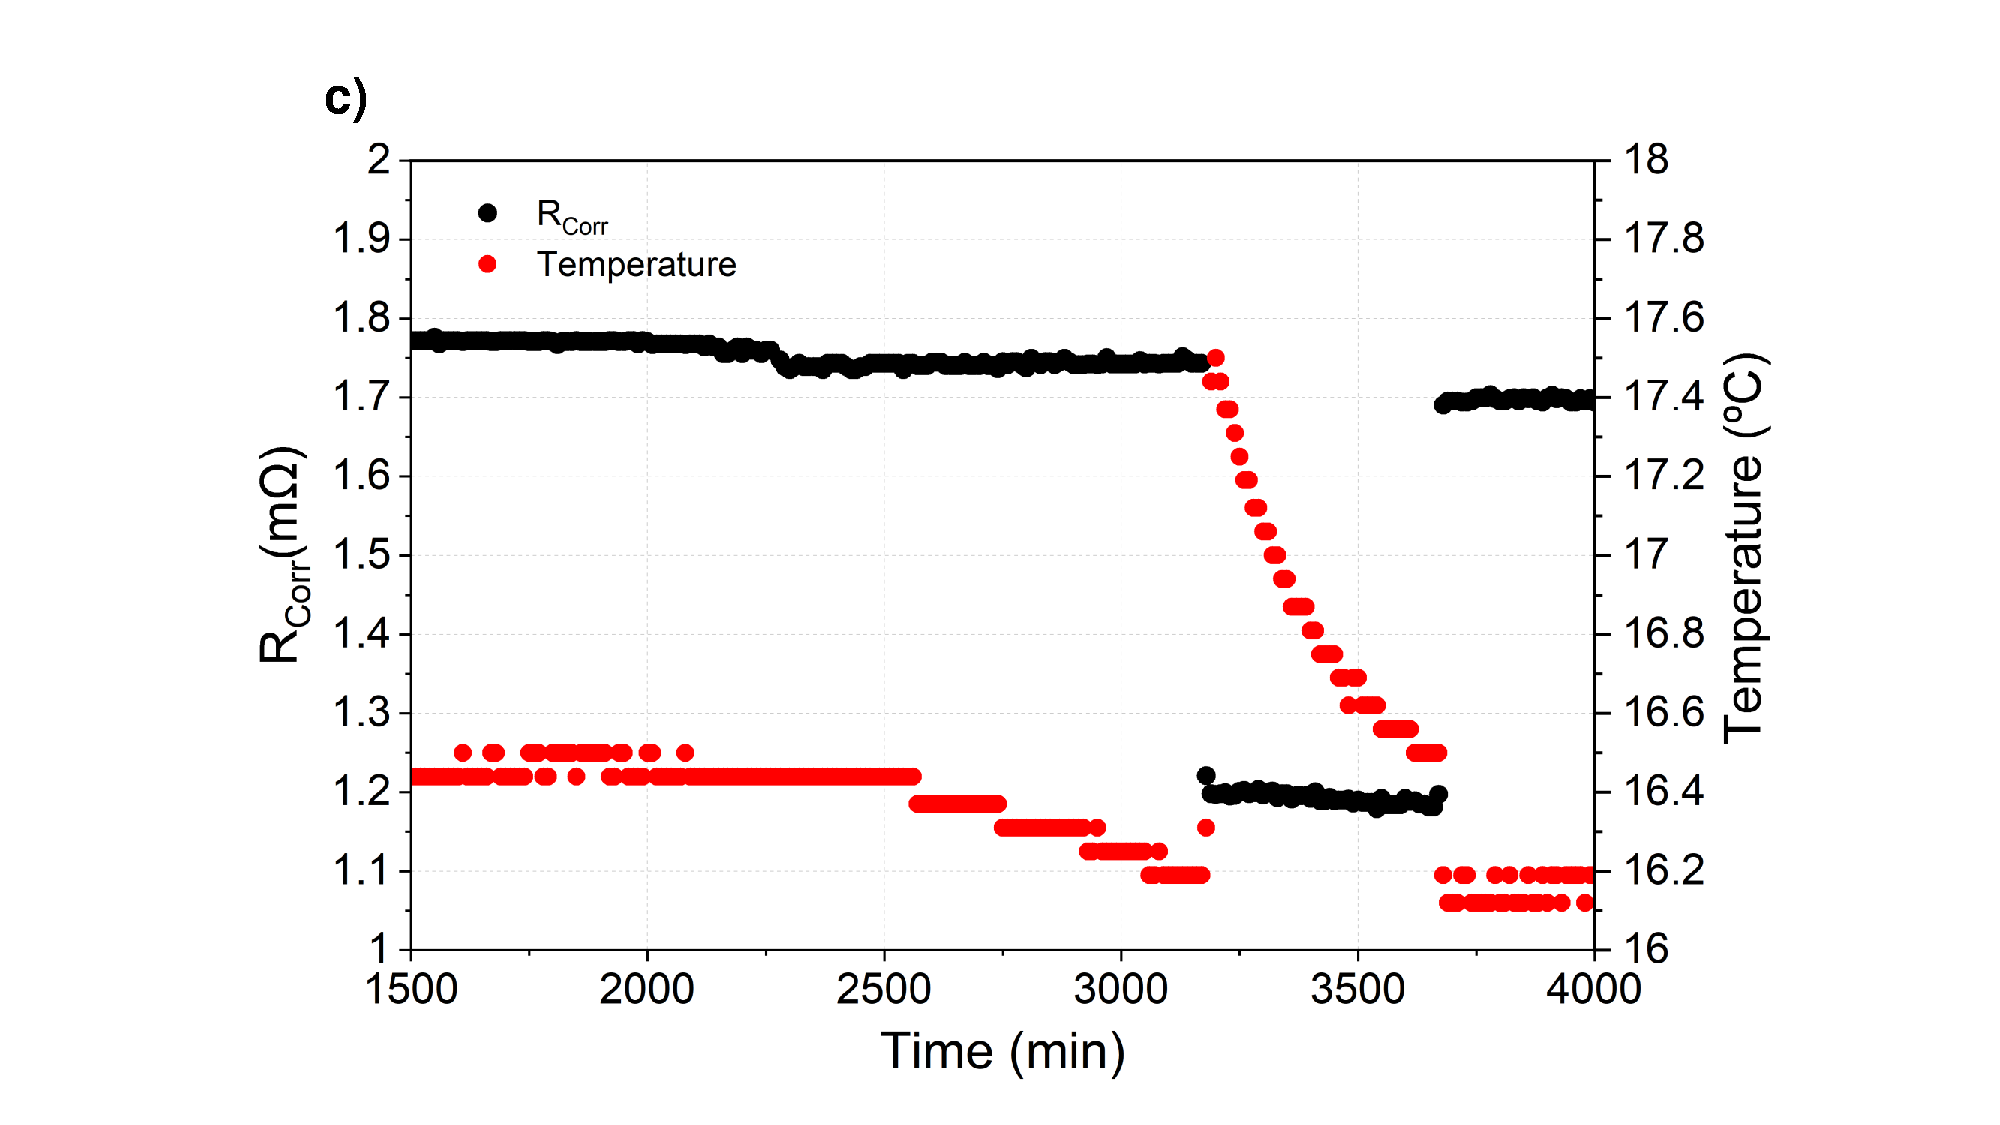
\includegraphics [trim = 40mm 0mm 40mm 10mm, clip, width=1\columnwidth]{images/fig10_2_v4.pdf}}
\subfigure{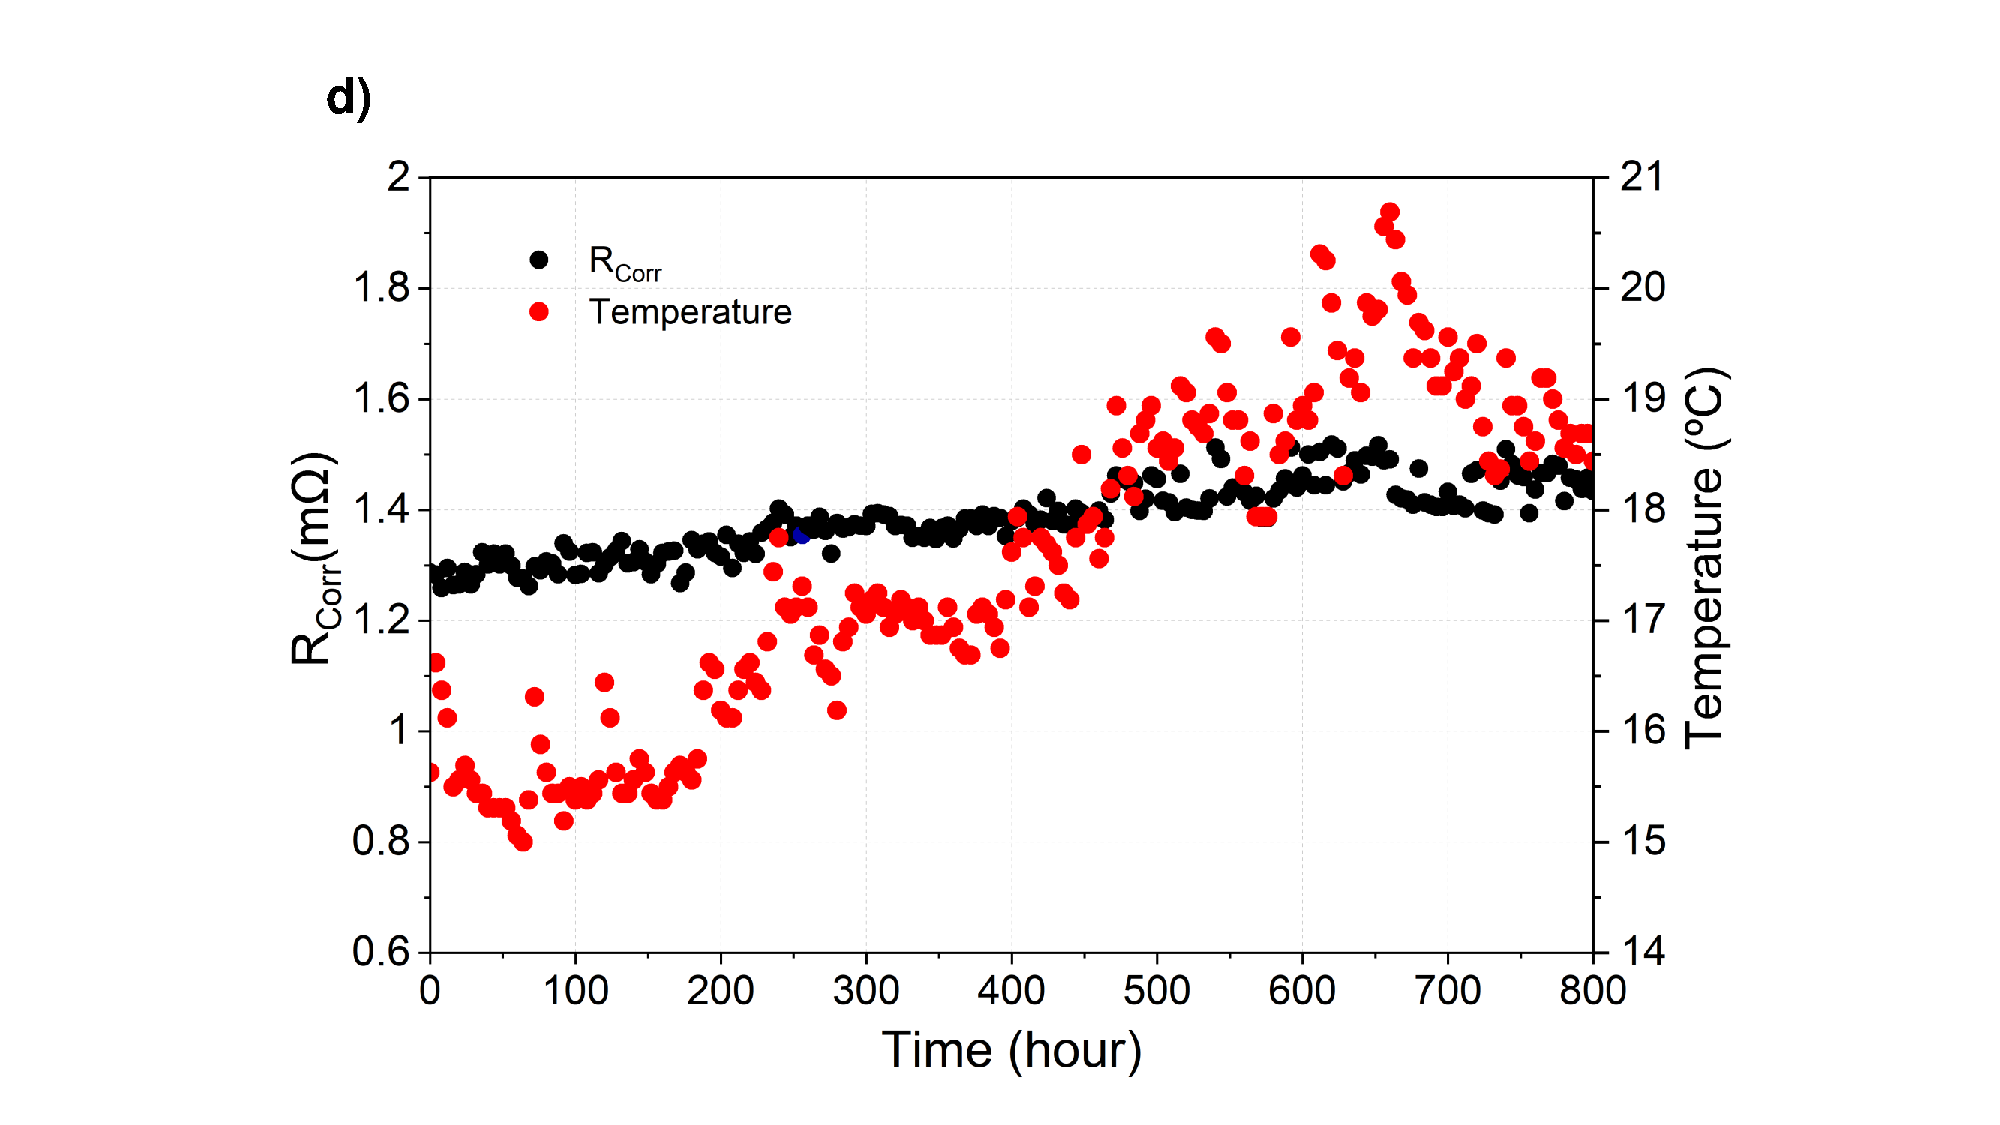
\includegraphics [trim = 44mm 0mm 40mm 10mm, clip, width=1\columnwidth]{images/fig10_3_v4.pdf}}
%\hfill
\caption{Measurements of the resistance of the R5 HSLA steel tube in two different corrosive environments. (a) First, the sensor was placed inside a $1$\,m$^{3}$ pool filled with salt water at concentration of $35$\,$\nicefrac{g}{L}$. The sensor is connected with a rugged version of the System Head and immersed $0.5$\,m bellow the surface. The System Head is directly connected to a Raspberry Pi 4B (RPB4). Samples were recorded every $10$\,min for two days with an extraction during the second day. (b) Afer that, a copy of the sensor was placed in the Tecnalia's HarshLab facility (Cantabrian Sea, $1.8$\,km offshore) $2$\,m bellow the sea surface. The System Head is connected to a GSM platform able to upload data (resistance and temperature of the tube, status of the System Head and possible errors) every $4$ hours. (c) Plot of the resistance and temperature recorded during $2$ days when the sensor is in the environment depicted in (a). The values of the resistance are already corrected in temperature with equation~\ref{eq:realRx}. The sensor was extracted from the pool for mechanical around minute $3210$. The dispersion of the measurements was $\pm2.05$\,$\mu\Omega$. (d) Plot of the resistance and temperature recorded during $30$ days when the sensor is in the environment depicted in (b). The values of the resistance are also corrected in temperature. The dispersion observed is $\sim$\,$\pm11.5$\,$\mu\Omega$.}
%\vspace{0.5cm}
\label{fig:poolMeas}
\end{figure}

In order to test the performance of the device presented here, a replica of the previously described and studied prototype was immersed $1.8$\,km offshore and $2$\,m deep in the Cantabrian Sea. The system (head and sensor connected to a GSM+battery station) was deployed in the Tecnalia's HarshLab facility as depicted in figure\,\ref{fig:poolMeas}\,(b). Resistance and temperature data were recorded for $30$ days every $4$ hours and sent to a ground server via GSM. The consumption of the prototype was $300$\,mA during measurement time (2 minutes) and dropped to less than $1$\,mA between measurements.

Figure\,\ref{fig:poolMeas}\,(d) shows the evolution of resistance (once corrected as explained in section~\ref{ssec:measSaltWat}) and temperature during the experiment. The observed dispersion was in the range of $\pm12\mu\Omega$ which corresponds to six times the dispersion observed with the prototype immersed in the \textit{inhouse} pool. The resultant minimum observable corrosion rate is $\sim$\,$1.1\nicefrac{\mu m}{yr}$, which is still a considerable improvement compared with other undersea corrosion devices~\cite{Yang2008} and commercial ER sensors. 

In addition to the noise observed in the prototype discussed in section~\ref{ssec:measSaltWat}, there is an extra source of uncertainty that degrades the performance of the sensor. The observed noise in the resistance measurement comes from fluctuations in the power supply in the GSM+battery station. This station is battery powered (charged by solar panels) and the delivered power is unregulated. The power goes to a standard voltage regulator in the sensor body and the power lines are attached directly to the $\mu$controller and the ADC. No stabilization capacitors have been used in this prototype in order to keep the power consumption at minimum. Therefore, the reference voltage for the ADC is not conveniently defined resulting in an increment of the noise.

\section{Conclusions}
\label{sec:conclusions}
In this work, a highly sensitive undersea corrosion sensor has been presented and tested. It works with thin steel tubes, acting as a corrosion probe, attached to a watertight enclosure. Inside the enclosure, a $\mu$-controller based $\mu\Omega$-meter and temperature sensors take measurements of resistance and temperature of the tube in contact with water. The data logging is performed by a system head polling the sensor at a constant rate and sending the data to an onshore station via GSM. 

The system has been developed both as laboratory and open-field prototype with measured observable corrosion rates of $\sim$\,$0.46$ and $1.1$\,$\nicefrac{\mu m}{yr}$ respectively. The total consumption of the system is $\leq 3$\,$\nicefrac{mA}{h}$ in both cases, although power supply instabilities were detected in the measurements recorded with the field prototype. This issue might be arranged by adding a stronger supply regulation technique inside the sensor enclosure.

The system is still recording data in the \textit{inhouse} pool and the offshore Tecnalia's facility. Therefore, the reliability and durability of the design are still under test and will be reported in future contributions with additional effects observed in measurements.



\section*{Acknowledgment}

The authors want to thank to Pablo Benguria, Ph.D. for his skills as project manager and scuba diver





\bibliographystyle{IEEEtran}
\bibliography{bibTex/ieeeBibTex_MagAndCorr.bib}
%\vspace{-1cm}
\vskip -2\baselineskip plus -1fil
\begin{IEEEbiography}[{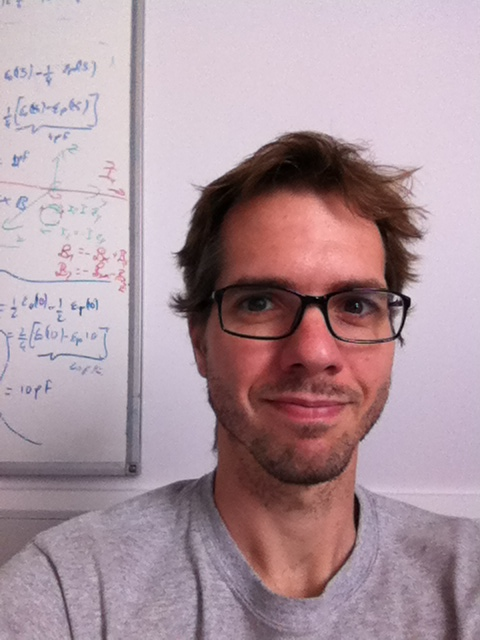
\includegraphics[width=1in,height=1.25in,clip,keepaspectratio]{images/JAV-Website-Photo.jpg}}]{Javier Alonso-Valdesueiro}
was born in Madrid, Spain in 1980. He received the Engineer's Degree from the University of Alcalá, Madrid, Spain in 2006 and the Ph.D. degree from the Polytechnic university of Catalonia, Barcelona, Spain in 2011.
From $2012$ to $2019$ he has been developing electronic instrumentation for NMR experiments, first at the C.E.A center in France, then, in the University of Southampton, and finally with a Marie Skłodowska-Curie Fellowship at the University of the Basque Country (UPV/EHU). He is currently main researcher at TECNALIA Research and Innovation in the Materials and Processes area.  His interests include MRI, RF novel hardware and methodologies, electronic instrumentation and harsh-condition sensing technologies.
\end{IEEEbiography}
\vskip -2\baselineskip plus -1fil
%\vspace{-1.5cm}
\begin{IEEEbiography}[{
\includegraphics[width=1in,height=1.25in,clip,keepaspectratio]{images/inyaki.jpg}}]{Iñaki Madinabeitia}
was born in Oñati (Gipuzkoa), Spain in 1990. He obtained his double degree in Physics and Electronic engineering from the University of the Basque Country (UPV/EHU). After a brief internship at the CIC nanoGUNE he completed his Master degree in Renewable Energies and Energy Sustainability at the University of Barcelona (UB). Since February 2017 he is a PhD student at CIC energiGUNE and Tecnalia, in the Structure and Surface Analysis group. He is currently working as an electronic engineer at TECNALIA.
\end{IEEEbiography}
\vskip -2\baselineskip plus -1fil
\begin{IEEEbiography}[{
\includegraphics[width=1in,height=1.25in,clip,keepaspectratio]{images/ISP-Photo.jpg}}]{Iñigo Santos-Pereda}
was born in Bilbao (Bizkaia), Spain in 1992. He received his degree on Chemistry from the University of the Basque Country (UPV/EHU), Leioa, Spain in 2015 and his MsC degree on Science of New Materials from the University of Cantabria and the University of the Basque Country (UPV/EHU) in 2016. Currently, he is a Ph.D. student focused on the development of new hardware and sensing methodology for corrosion monitoring in offshore facilities.
\end{IEEEbiography}
\vskip -2\baselineskip plus -1fil
\begin{IEEEbiography}[{
\includegraphics[width=1in,height=1.25in,clip,keepaspectratio]{images/jb.jpg}}]{Jean-Baptiste Jorcin}
Jean-Baptiste Jorcin received his degree in Chemistry from the Université de Savoie, his master degree in chemistry and Material engineering from the Université du Québec à Montréal, Université du Sud and was awarded with his PhD degree in material science and engineering by the Institut National Polytechnique de Toulouse. He stayed as a postdoctoral researcher in the SURF group from the Vrije Universiteit Brussel for three years, and 8 months at the Instituto Superior Tecnico,  were he worked on various corrosion related topics. Nowadays, he is working at TECNALIA in the Energy and Environment division where he is participating, and leading projects connected to the corrosion topic.
\end{IEEEbiography}
\vskip -2\baselineskip plus -1fil
\begin{IEEEbiography}[{
\includegraphics[width=1in,height=1.25in,clip,keepaspectratio]{images/Esther Acha.jpg}}]{Esther Acha-Peña}
Chemical Engineer in 2006 and PhD with international mention in Advanced Materials Engineering from the UPV/EHU in 2013, with a 6-month pre-doctoral stay at the Energy Research Center of the Netherlands (ECN, The Netherlands) and two post-doctoral stays at the ECN (2 months) and at the Norwegian Science and Technology University NTNU (Norway) (3 months). She has been a lecturer in the Dept. of Chemical Engineering and Environment of the UPV/EHU since 2010, and permanent lecturer since 2018. Her lines of research are focused on alternative fuels and energy by thermal treatment of waste among others.
\end{IEEEbiography}

\end{document}
